\documentclass{report}

\usepackage{blindtext}

\usepackage{amsmath}

\usepackage{graphicx}
\graphicspath{{images/}{../images/}}

\usepackage[utf8]{inputenc}

\usepackage[nottoc]{tocbibind}

\usepackage{listings}
\lstset{language=C++,
    frame=l,
    %breakindent=0.1\textwidth,
    breaklines=true,
    numbers=left,
    numberstyle=\scriptsize\ttfamily,%\footnotesize,
    showspaces=false,
    showtabs=false,
    showstringspaces=false,
    basicstyle=\scriptsize\ttfamily,
    keywordstyle=\color{blue}\scriptsize\ttfamily,
    stringstyle=\color{green}\scriptsize\ttfamily,
    commentstyle=\color{gray}\scriptsize\ttfamily,
    morecomment=[l][\color{purple}]{\#}
}

\usepackage{multirow}

\usepackage{textcomp}
\usepackage{pgfplots}

\usepackage{algorithm}
\usepackage{algpseudocode}

\usepackage{chngcntr}
\counterwithout{figure}{chapter}
\counterwithout{equation}{chapter}

\pgfplotsset{width=10cm,compat=1.9}

\setcounter{secnumdepth}{5}

\usepackage{pgfplotstable}
\usepgfplotslibrary{groupplots}

\usepackage[section]{placeins}

\usepackage{hyperref}

\usepgfplotslibrary{fillbetween}

\usepackage[autostyle]{csquotes}
\usepackage{caption}
\usepackage{subcaption}

\usepackage{xcolor}
\usepackage{varwidth}


\begin{document}

\begin{titlepage}
    \centering
    \includegraphics[scale=0.35]{logo.jpg} \par\vspace{1cm}
    {\scshape\LARGE Umeå University \par}
    {\scshape\Large Department of Computing Science\par}
    \vspace{1cm}
    {\scshape\Large Efficient algorithms\par}
    {\scshape\large 5DV182\par}
    \vspace{1.5cm}
    {\huge\bfseries Cocke–Younger–Kasami algorithm analysis\par}
    \vspace{2cm}
    {\Large\itshape Thomas Ranvier\par}
    \vfill 
    {\large supervised by\par}
    Franck \textsc{Drewes}
    \vfill 
    {\large November 04, 2018\par}
\end{titlepage}


\chapter*{Abstract}
This paper presents six different implementations of the Cocke-Younger-Kasami algorithm (CYK algorithm for short).
The first one is a naive version, it uses the Divide and conquer approach and has a complexity of $O(3^n)$.
The other implementations make use of Dynamic programming, there are two versions using bottom-up approach and the others use the top-down method, they all have a complexity of $O(n^3)$.

The four first parsers are classic implementations of the CYK algorithm using different programming methods, the last two have some specialities.
After the presentation of the implementations and the analysis of the different complexities a chapter is focused on experimentations with the four first parsers using diverse context-free grammars in the Chomsky normal-form.

The implementation of a parser able to make use of linear grammars with a running time of $O(n^3)$ and based on the top-down implementation is presented.
Experimentations and comparisons with the results of the four previous parsers are made.

A parser that automatically corrects the input string in order to make it match the given grammar (when possible) in $O(n^3)$ is presented.
This parser is based on the top-down initial implementation, it suggests to the user a correction of the initial string and indicates the number of character modifications and character deletions that were needed to reach total correctness.


\tableofcontents

\chapter*{Introduction}
\addcontentsline{toc}{chapter}{Introduction}
This is the report of the efficient algorithms assignment on the CYK parser.

The point of the assignment was firstly to discover and implement the CYK algorithm using several development approaches.
Then the goal was to experiment with the implementations and compare their efficiencies for diverse context-free grammars in the Chomsky normal-form.

After that the task was to design a parser that can work with linear grammars, to implement it and then to experiment with it in order to compare its efficency to the other parsers.

Then the final goal was to design and implement a parser that does not simply return true if the string is part of the language and false otherwise, but corrects the input string and returns a proposed correction with the needed number of character modifications and deletions.


\chapter{Context}

\section{Context-free grammar}

Context-free grammars are part of the Chomsky hierarchy \cite{grammars_hierarchy, grammars} and can be defined as a quadruple $G = (N, \Sigma, P, S)$ that consists of the following components:

\begin{itemize}
    \item[$-$] $N$ is a finite set of \textit{non-terminal} variables.
    \item[$-$] $\Sigma$ is a finite set of \textit{terminal} variables.
    \item[$-$] $P$ is a finite set of \textit{production rules}, also called \textit{rewrite rules}, it specifies a symbol substitution that can be recursively performed to generate new symbol sequences. In an unrestricted grammar, which is the most general form of the Chomsky hierarchy, a production is of the form $u \to v$ where $u$ and $v$ are arbitrary strings of \textit{terminals} and \textit{non-terminals}.
    \item[$-$] $S \in N$ is a distinguished symbol that is the \textit{start symbol}, also called the \textit{sentence symbol}.
\end{itemize}

The language $L(G)$ is the language generated by the grammar G \cite{intro_automata}.
To generate a string of the language, one begins with a string consisting of only a single start symbol, and then successively applies the rules (any number of times, in any order) to rewrite this string. 
This stops when we obtain a string containing only terminals.
The language consists of all the strings that can be generated in this manner.

The same process can be applied backward to check weither a given string can be generated by the grammar or not.

\subsection{Description of the Chomsky normal-form}

Here is an example of a context-free grammar in the Chomsky normal-form:

\begin{align*} 
&S \to AB|BC\\
&A \to BA|a\\
&B \to CC|b\\
&C \to AB|a
\end{align*}

The grammar can be described as a finite set of production rules, in those productions we can find four types of symbols:

\begin{itemize}
    \item[$-$] The `$\to$' symbol is what seperates the left-hand from the right-hand(s) of the rules.
    \item[$-$] In this grammar every single uppercase letter is a \textit{non-terminal} variable.
    \item[$-$] The \textit{terminals} are primitive symbols, they can only be found on the right-hand of a production.
    \item[$-$] A left-hand is constitued of one \textit{non-terminal}, it can relate to one or several right-hands seperated by the `$|$' symbol. A right-hand is constitued either by one \textit{terminal} or a pair of \textit{non-terminals}.
\end{itemize}

Here S, A, B, and C are \textit{non-terminals}, a and b are \textit{terminals} and S is the \textit{start symbol}.

\subsection{Convert grammar to Chomsky normal-form}

Sometimes it is needed to convert a context-free grammar to the Chomsky normal-form.
Later in this report is presented an algorithm that follows the next pseudo-code in order to automaticly convert a given context-free grammar into the Chomsky normal-form.
\\
\\
For example this is how to convert the following grammar:

\begin{align*} 
&S \to S+P|P\\
&P \to P*C|C\\
&C \to (S)|0|1\\
\end{align*}

\begin{enumerate}
    \item The first thing to do is to eliminate the \textit{start symbol} from the right-hands of the grammar by replacing the \textit{start symbol} by a new one (some labels have been modified):
        \begin{align*} 
        &S \to A\\
        &A \to A+B|B\\
        &B \to B*C|C\\
        &C \to (A)|0|1\\
        \end{align*}

    \item Then the goal is to replace the \textit{terminals} that are not the only symbols on the right-hand by a new \textit{non-terminal}:
        \begin{align*} 
        &S \to A        &P \to +\\
        &A \to APB|B    &M \to *\\
        &B \to BMC|C    &L \to (\\
        &C \to LAR|0|1  &R \to )\\
        \end{align*}
    
    \item The next step is to delete the right-hands with more than 2 \textit{non-terminals} by adding \textit{non-terminals} that will relate to a pair:
        \begin{align*} 
        &S \to A        &F \to AR\\
        &A \to AD|B     &P \to +\\
        &B \to BE|C     &M \to *\\
        &C \to LF|0|1   &L \to (\\
        &D \to PB       &R \to )\\
        &E \to MC\\
        \end{align*}

    \item At last it is needed to eliminate the unit rules, those are the right-hands in which there is one \textit{non-terminal} alone:
        \begin{align*} 
        &S \to AD|BE|LG|0|1 &F \to AR\\
        &A \to AD|BE|LG|0|1 &P \to +\\
        &B \to BE|LG|0|1    &M \to *\\
        &C \to LF|0|1       &L \to (\\
        &D \to PB           &R \to )\\
        &E \to MC\\
        \end{align*}

\end{enumerate}

\section{CYK algorithm}

The CYK algorithm is a parser for context-free grammar, it is named after its inventors, John Cocke, Daniel Younger and Tadao Kasami.
The algorithm takes a string and a context-free grammar as input and determines if the string is part of the language of the grammar or not.
It uses the backward process explained in the presentation of section 1.1.

Context-free grammar parsers can be used for example in computer sciences to check code structure in compilers or in biology for DNA and RNA strings analysis.

\section{Diverse development approaches}

The goal of the assignment is to implement CYK parsers using different development approaches in order to compare the efficiency of those.
In this section the three used development methods are briefly presented.

\subsection{Divide and conquer}

Divide and conquer is an algorithmic strategy that consists in recursively breaking down a problem into several others, and do so until the problems become easy enough to solve. 
The obtained results are then combined in order to solve the initial problem.
\\
\\
Those are the steps of the general structure of that strategy:

\begin{enumerate}
    \item Divide the problem instance given as input into smaller instances.
    \item Recursively compute the results for those smaller instances.
    \item Assemble the recursively obtained results into a result for the entire input and return it.
\end{enumerate}

\subsubsection{Recurrence relation}

It is possible to find a function that satisfies the recurrence relation of the divide and conquer strategy.
Let's suppose that a recursive algorithm divides a problem of size $n$ into $a$ sub-problems, where each sub-problem is of size $\dfrac{n}{b}$
Suppose also that $g(n)$ is the total time needed to create the sub-problems and combine their results.

Then we can define $f(n)$, being the number of operations needed to solve the problem of size $n$, as:
$$
f(n) = a * f(\dfrac{n}{b}) + g(n)
$$

\subsubsection{Master theorem}

The Master theorem for the divide and conquer recurrences provides an asymptotic analysis of the complexity, using the Big O notation.
It allows one to solve $f(n)$ depending on three different cases.
\\
\\
Now that we have the function $f(n)$ we suppose that $g(n) = \Theta(n^d)$.
\\
\\
Then the master theorem is:
$$
f(n) = 
\begin{cases}
    \Theta(n^d) &\text{if } a < b^d\\
    \Theta(n^dlog(n)) &\text{if } a = b^d\\
    \Theta(n^{log_b(a)}) &\text{if } a > b^d\\
\end{cases}
$$

Here the first case is when it is possible to ignore the solving of the subproblems before the creation and combination of the sub-problems. The running time is then the time needed to create and combine the sub-problems, $g(n) = \Theta(n^d)$.

The second case is when it is not possible to ignore anything.

The final case is when it is possible to ignore the creation and combination of the sub-problems. The running time is then the time needed to solve $a^{log_b(n)}$ subproblems of size 1.

\subsection{Dynamic programing}

Dynamic programing is an algorithmic paradigm that solves a given complex problem by breaking it down into subproblems and storing the results of those subproblems to avoid computing the same results again.

\subsubsection{Top-down approach}

The top-down approach is similar to the divide and conquer approach, the initial problem is recursively broken down into several sub-problems.
The difference is that in this approach a global variable memorize every computed result. 
In that way when the program runs into a known problem the memorized result is directly returned.
The program generally computes less operations and goes less deep in the recursion than the divide and conquer method.

\subsubsection{Bottom-up approach}

The bottom-up approach consists in solving the simplest sub-problems first, memorizing every computed result, and then going up solving bigger and bigger sub-problems until it can solve the initial problem.
This approach is a way to avoid recursion, which saves some memory, but on the other hand it can sometimes solve sub-problems that will never be used to solve the initial problem, which is a waste of time.

A good analogy for the bottom-up design are building blocks, indeed you have to start assembling the most little pieces together in order to construct bigger ones that you will then assemble to get the final result.



\chapter{Implementations of the different parsers}

\section{Grammar}

This is the description of the Grammar class as it has been used for the general experimentations that can be found in the chapter 3.
A more efficient version that can handle linear and Chomsky normal-form grammars has been implemented and is presented later in this report.

The different productions of the context-free grammar are given by the user through a file following the same pattern as the example of section 1.1.2.
\\
\\
The program uses the following conventions:
\begin{itemize}
    \item[$-$] Every \textit{non-terminal} is a single uppercase letter.
    \item[$-$] Every \textit{terminal} is a single other ASCII character.
    \item[$-$] The right-hand is composed of one or several groups, each group is either a pair of \textit{non-terminals} or a single \textit{terminal}.
\end{itemize}

When the program comes accross an uppercase letter it automaticly transorms it into an index beginning from 0, so 'A' becomes 0, 'B' becomes 1, etc.
\\
\\
My program then fills three variables:
\begin{itemize}
    \item[$-$] The variable `non\_terminals' is a string, when a new \textit{non-terminal} is read from the file it is converted as described above and then added as a character to the variable. This variable will then make it easy and efficient to access the rules.
    \item[$-$] The variable `non\_terminal\_rules' is a three dimensional array of integers.
        \begin{enumerate}
            \item The first dimension has the size of the latin alphabet: 26, each line of this dimension will allow access to the non-terminal rules of the corresponding \textit{non-terminal}, using the converted values stored in `non\_terminals'.
            \item The second dimension allows access to the different pairs of \textit{non-terminals}.
            \item The third dimension has a size of 2, it represents the pair of \textit{non-terminals}.
        \end{enumerate}
    \item[$-$] The variable `terminal\_rules' is a two dimensional array of integers.
        \begin{enumerate}
        \item The first dimension has the size of the latin alphabet, each line of this dimension allows access to the terminal rules of the corresponding \textit{non-terminal}.
        \item The second dimension allows access to the different \textit{terminals} related to that \textit{non-terminal}.
        \end{enumerate}
\end{itemize}

The point of seperating the \textit{non-terminal} rules from the \textit{terminal} ones in two variables is that they are always accessed on different cases. It would then slow down the processus to always have to differenciate them from one another.

\section{Naive parser}

The naive implementation uses the divide and conquer approach, 

\FloatBarrier
\begin{algorithm}
    \caption{Naive parser}
    \label{parse}
    \begin{algorithmic}[1]
        \State $s \gets input\_string$
        \Procedure{parse}{$var, i, j$} \Comment{Recursive parser function}
            \If{$i == j - 1$}
                \ForAll{$t \in terminal\_rule[var]$}
                    \If{$t == s[i]$}
                        \State \textbf{return} $true$
                    \EndIf
                \EndFor
            \Else
                \ForAll{$nt \in non\_termial\_rules[var]$}
                    \For{$k \gets i + 1; k < j$}
                        \If{$parse(nt[0], i, k) \land parse(nt[1], k, j)$}
                            \State \textbf{return} $true$ 
                        \EndIf
                    \EndFor
                \EndFor
            \EndIf
            \State \textbf{return} $false$
        \EndProcedure
    \end{algorithmic}
\end{algorithm}
\FloatBarrier

\subsection{Complexity of the algorithm}

To find the complexity of this algorithm one can draw recursion trees for small values of $n$ and find the following sequence: $0, 2, 8, 26, 80$\dots
After some research it is possible to find out that this sequence corresponds to the formula $3^{n - 1} - 1$ \cite{naive_formula}.

The resulting complexity of this algorithm is then $O(3^n)$.

\section{Top-down parser}

The top-down implementation is almost the same as the naive one, except that there is here a global variable that memorize every computed results.

\FloatBarrier
\begin{algorithm}
    \caption{Top-down parser}
    \label{parse}
    \begin{algorithmic}[1]
        \State $table$ is a 3d array of 0
        \State $s \gets input\_string$
        \Procedure{parse}{$var, i, j$} \Comment{Recursive parser function}
            \If{$table[var, i, j] != 0$}
                \State \textbf{return} $(table[var, i, j] == 1)$
            \EndIf
            \If{$i == j - 1$}
                \ForAll{$t \in terminal\_rule[var]$}
                    \If{$t == s[i]$}
                        \State $table[var, i, j] \gets 1$
                        \State \textbf{return} $true$
                    \EndIf
                \EndFor
            \Else
                \ForAll{$nt \in non\_terminal\_rules[var]$}
                    \For{$k \gets i + 1; k < j$}
                        \If{$parse(nt[0], i, k) \land parse(nt[1], k, j)$}
                            \State $table[var, i, j] \gets 1$
                            \State \textbf{return} $true$ 
                        \EndIf
                    \EndFor
                \EndFor
            \EndIf
            \State $table[var, i, j] \gets 2$
            \State \textbf{return} $false$
        \EndProcedure
    \end{algorithmic}
\end{algorithm}
\FloatBarrier

\subsection{Complexity of the algorithm}

To compute the running-time of the top-down algorithm we can count the number of cells in the memoization table and multiply it by the complexity of the inner loops of the algorithm.
This will give an upper bound of the complexity.
The loops that go through the grammar are ignored, the size of the table is $n^2$, with $n$ the size of the input string, the complexity of the parse function without any recursion is $O(n)$, so the complexity of the top-down parser is $O(n * n^2) = O(n^3)$.

\section{Bottom-up parser}

For this parser there are two possible implementation versions, one uses a boolean table and the other one uses a string table, their process are slightly different and they give different results in term of iterations and running time.

In the first approach the goal is to complete a triangular matrix, when the matrix is fully completed it watches the last cell and if it finds the \textit{start symbol} in it it returns true, otherwise it returns false.
That version is called the `string' bottom-up parser in this report.

\FloatBarrier
\begin{algorithm}
    \caption{`String' bottom-up parser}
    \label{parse}
    \begin{algorithmic}[1]
        \Procedure{parse}{$s$} \Comment{Iterative parser function}
            \State $matrix$ is a 2d array of empty strings
            \State $step \gets 0$
            \For{$i \gets 0; i < s.length()$}
                \ForAll{$var \in non\_terminals$}
                    \ForAll{$t \in terminal\_rules[var]$}
                        \If{$t == s[i]$}
                            \State Add $var$ to $matrix[step, i]$ if not already inside
                        \EndIf
                    \EndFor
                \EndFor
            \EndFor
            \State $step \gets step + 1$
            \While{$s.length() - step > 0$}
                \For{$i \gets 0; i < s.length() - step$}
                    \For{$j \gets 0; j < step$}
                        \State $r \gets check\_combs(matrix[j, i], matrix[step - (j + 1), i + j + 1])$
                        \State Add $r$ to $matrix[step, i]$ if not already inside
                    \EndFor
                \EndFor
                \State $step \gets step + 1$
            \EndWhile
            \State \textbf{return} is the start symbol in $matrix[s.length() - 1, 0]$ ?
        \EndProcedure
        \Procedure{check\_combs}{$cell\_1, cell\_2$}
            \State $result$ is an empty string
            \For{$i \gets 0; i < cell\_1.length()$}
                \For{$j \gets 0; j < cell\_2.length()$}
                    \State $production \gets cell\_1[i] . cell\_2[j]$
                    \If{$production$ is in the $non-terminal\_rules$}
                        \State Add the left hand of the matching rule to $result$
                    \EndIf
                \EndFor
            \EndFor
            \State \textbf{return} $result$
        \EndProcedure
    \end{algorithmic}
\end{algorithm}
\FloatBarrier

In the second approach the goal is to complete a boolean table, then it looks in a specific cell and returns the result.
That parser is called the `boolean' bottom-up parser in this report.

\FloatBarrier
\begin{algorithm}
    \caption{`Boolean' bottom-up parser}
    \label{parse}
    \begin{algorithmic}[1]
        \Procedure{parse}{$s$} \Comment{Iterative parser function}
            \State $matrix$ is a 3d array of false booleans
            \State $step \gets 0$
            \For{$i \gets 0; i < s.length()$}
                \ForAll{$var \in non\_terminals$}
                    \ForAll{$t \in terminal\_rules[var]$}
                        \If{$t == s[i]$}
                            \State $matrix[0, i, var] \gets true$
                        \EndIf
                    \EndFor
                \EndFor
            \EndFor
            \State $step \gets step + 1$
            \While{$s.length() - step > 0$}
                \For{$i \gets 0; i < s.length() - step$}
                    \For{$j \gets 0; j < step$}
                        \ForAll{$var \in non\_terminals$}
                            \ForAll{$t \in terminal\_rules[var]$}
                                \State $bool\_1 \gets matrix[j, i, t[0]]$
                                \State $bool\_2 \gets matrix[step - j - 1, i + j + 1, t[1]]$
                                \If{$bool\_1 \land bool\_2$}
                                    \State $matrix[step, i, var] \gets true$
                                \EndIf
                            \EndFor
                        \EndFor
                    \EndFor
                \EndFor
                \State $step \gets step + 1$
            \EndWhile
            \State \textbf{return} $matrix[s.length() - 1, 0, start\_symbol\_index]$
        \EndProcedure
    \end{algorithmic}
\end{algorithm}
\FloatBarrier

The `boolean' implementation needs a predictable amount of iterations for a given grammar to parse a string, no matter what pattern this string follows.
The `string' one on the other hand needs a various number of iterations depending on the pattern of the input string.

\subsection{Complexity of the algorithms}

The two algorithms above have the same complexity, to determine it it is needed to look at the inner loops of the algorithms.
For both of them if the grammar loops are ignored the complexity is $O(n + n^3) = O(n^3)$.

\subsection{Expression of the number of iterations}

For the `boolean' bottom-up parser it is possible to predict the exact number of iterations that it will compute, indeed unlike the naive and top-down versions there is no recursion that denies us to anticipate it.

It is possible to translate the `for' and `while' loops into a mathematical expression:
\begin{equation} \label{eq:bottom-up_iterations_with_sum}
    iterations = n \cdot gt + \sum_{k = 1}^n (n - k) \cdot k \cdot gnt
\end{equation}

With:
\begin{itemize}
    \item[$-$] $n$ being the size of the input string.
    \item[$-$] $gt$ being the number of terminal rules: the number of \textit{terminals} on the right-hands of the grammar.
    \item[$-$] $gnt$ being the number of non terminal rules: the number of \textit{non-terminals} pairs on the right-hands of the grammar.
\end{itemize}

With such an expression it will be easier to justify the observed results in the `boolean' bottom-up parser case.

But the equation \ref{eq:bottom-up_iterations_with_sum} has an issue, it is not a polynomial function, which denies one from displaying it in a plot for example.
To get a real mathematical expression it is possible to use the Faulhaber's formulas that allows one to translate a sum into a polinomial function:

\begin{align*}
    iterations &= n \cdot gt + \sum_{k = 1}^n (n - k) \cdot k \cdot gnt\\
    &\Leftrightarrow n \cdot gt + gnt \cdot \sum_{k = 1}^n n \cdot k - k^2\\
    &\Leftrightarrow n \cdot gt + gnt \cdot (n \cdot \sum_{k = 1}^n k - \sum_{k = 1}^n k^2)\\
    &\Leftrightarrow n \cdot gt + gnt \cdot (\dfrac{n^2 \cdot (n + 1)}{2} - \dfrac{n \cdot (n + 1) \cdot (2 \cdot n + 1)}{6})
\end{align*}

The final expression is the following:
\begin{equation} \label{eq:bottom-up_iterations}
    iterations = n \cdot gt + \dfrac{gnt}{6} \cdot (3 \cdot n^2 \cdot (n + 1) - n \cdot (n + 1) \cdot (2 \cdot n + 1))
\end{equation}

The function above is a general expression of the number of iterations that the boolean bottom-up parser will have to do in order to parse a string of size $n$ for a grammar possessing $gt$ \textit{terminals} and $gnt$ pairs of \textit{non-terminals} on its right-hands.

With such function one can represent the behaviour of the number of iterations when the number of \textit{non-terminals} $gnt$ increases and the strings sizes $n$ too.

\FloatBarrier
\begin{figure}[h]
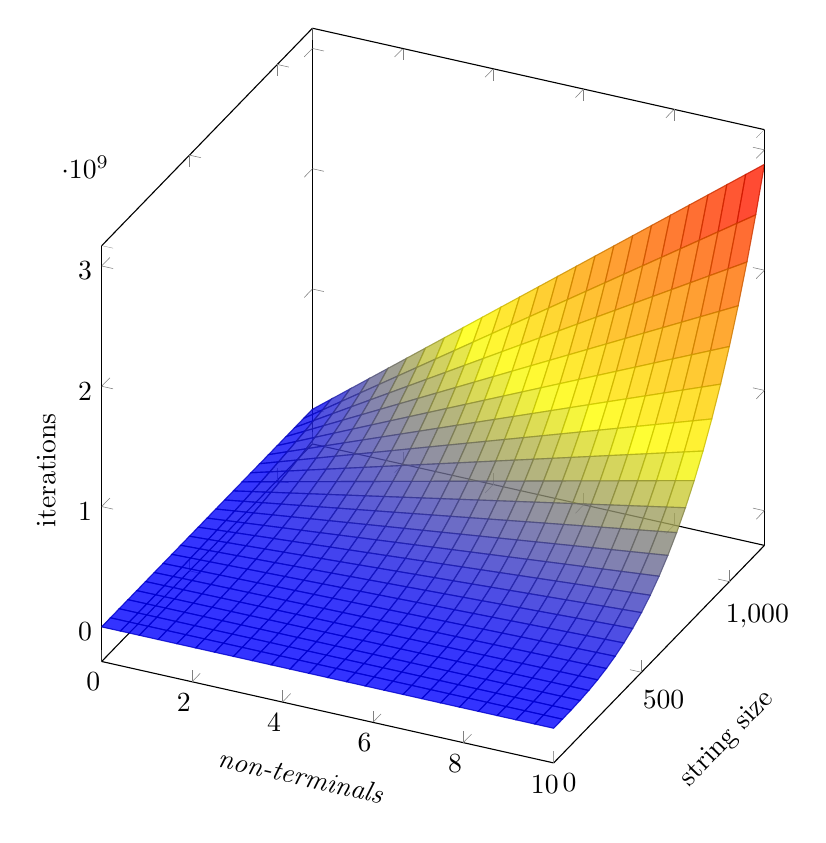
\begin{tikzpicture}
\begin{axis}[
    xlabel=\textit{non-terminals},
    ylabel=string size,
    zlabel=iterations,
    xlabel style={sloped like x axis},
    ylabel style={sloped},
    height=0.9\textwidth
]
\addplot3[
    surf,
    opacity=0.8,
    samples=25, samples y=25,
    domain=0:10,domain y=0:1200
]
    {y*0 + ((x/6) * (3*y*y*(y+1) - (y*(y+1)*(2*y+1))))};
\end{axis}
\end{tikzpicture}
\caption{3D plot of the function \ref{eq:bottom-up_iterations}}
\end{figure}
\FloatBarrier

It is interesting to see on the 3d plot that for a fixed $gnt$ when $n$ increases the number of iterations increases following a power function which should be of the form $y = a \cdot x^3$, since the complexity of the bottom-up parser is $O(n^3)$.

On the other hand when $n$ is fixed and that $gnt$ increases the number of iterations increases following a linear function.
That can be explained by the fact that the \textit{non-terminals} represent only on loop in the parser, so if the amount of \textit{non-terminals} is changed the impact on the number of iterations is linear.



\chapter{Experimentations, comparisons and obtained results}

\section{Generation of the strings}

In order to make the experimentations easier the input strings are automaticaly generated using patterns.
Those patterns are put in a file by the user which allows him to quickly be able to experiment with different cases.
Then when the Enumeration class is instanciated it reads the patterns from the file and all the strings are generated and stocked in a vector, then the strings can be accessed easily from anywhere.

The patterns uses the following expression:
$$
c \string^ x \text{\textvisiblespace} d \string^ y
$$

Where $c$ is an ASCII character and $x$ is the number of time we add the character, a space separates each characters.
It is also possible not to renseignate $\string^ x$, then the character is added 1 time.

That method allows the user to generate new strings for different grammars very quickly.

\section{Experimentations}

In some of the experimentations the results of the naive parser will not be displayed, which means that it was not efficient enough to be interesting.

The results of the `boolean' bottom-up parser will be displayed only once per grammar since no matter the pattern of the input string it does not change the behaviour of this parser.
However its results might be used several times for a same grammar in order to use them as reference for the other parsers.

\subsection{Well balanced parentheses}
The grammar is the following:

\begin{align*} 
    &S \to SS|LA|LR\\
    &A \to SR\\
    &L \to (\\
    &R \to )
\end{align*}

With this grammar it is possible to demonstrate that the top-down parser needs less recursive calls when it can `detect' that the string does not match the grammar very quickly.

\subsubsection{Number of iterations/recursive calls for each parsers}

With this grammar two interesting cases will be considered:

\begin{enumerate}
    \item Any pattern starting with a right parenthese:
    $$
    patterns = 
    \begin{cases}
        )\string^ n\\
        ) \text{ } (\string^ n - 1\\
        )\string^ n - 1 \text{ } (\\
    \end{cases}
    $$
    Many other patterns corresponding to the same case could be found, as long as the first character is a right parenthese.
    This case is interesting because it is the case in which the top-down parser needs to solve the less sub-problems in order to parse the strings.
    
    For example if it parses a string of size $n$ based on one of the patterns above it will need to solve $2n - 1$ sub-problems to give the result.
    That information, while interesting, is not relevant to anticipate the running time of the parser since even if we know how many sub-problems the parser will solve it can need a very different amount of recursive calls.
    
    \item The other interesting case is the pattern `$(\string^ n$', that pattern is the worst that can be generated with this grammar for the top-down parser.

    With that pattern the top-down parser will need to solve $n^2 + \lfloor \dfrac{n}{2} \rfloor$ sub-problems to parse a string of size $n$.
\end{enumerate}

Of course as demonstrated in the section 2.4 with equation \ref{eq:bottom-up_iterations} the `boolean' bottom-up parser always needs the same amount of iterations for a string of size $n$ and a given grammar:

\begin{itemize}
    \item[$-$] $n = 500$
    \item[$-$] $gt = 2$
    \item[$-$] $gnt = 4$
\end{itemize}

$$
500 \cdot 2 + \dfrac{4}{6} \cdot (3 \cdot 500^2 \cdot (500 + 1) - 500 \cdot (500 + 1) \cdot (2 \cdot 500 + 1)) = \text{83,334,000 iterations}
$$

Which is indeed the number of iterations obtained when running the code.

The `string' bottom-up parser will also follow the same behaviour for any string pattern.

It is now possible to represent the anticiped behaviour that the `boolean' bottom-up parser will follow for both cases.

\FloatBarrier
\begin{figure}[h]
\centering
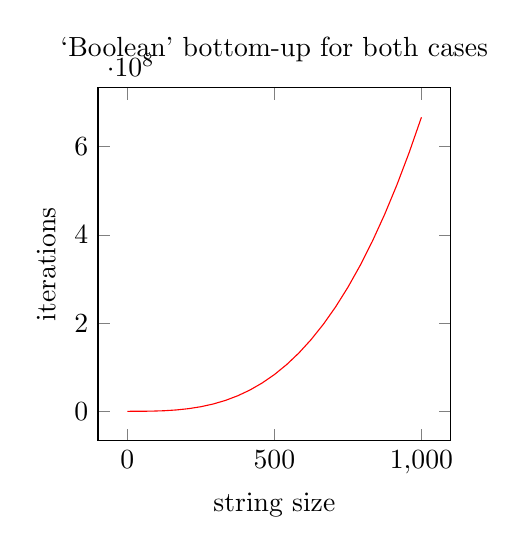
\begin{tikzpicture}
\begin{groupplot}[group style={group size=1 by 1},height=0.5\textwidth,width=0.5\textwidth, domain=0:1000]
    \nextgroupplot[title=`Boolean' bottom-up for both cases, ylabel=iterations, xlabel=string size]
    \addplot[red]{2 * x + ((4 / 6) * ((3 * (x^2) * (x + 1)) - (x * (x + 1) * ((2 * x) + 1))))};
\end{groupplot}
\end{tikzpicture}
\caption{Anticipation of the `boolean' bottom-up parser, grammar 1}
\end{figure}
\FloatBarrier

\subsubsection{Comparing the efficiency}

The first experimentation uses the case in which the strings are starting with a right patenthese: $)\string^ n$.

\FloatBarrier
\begin{figure}[h]
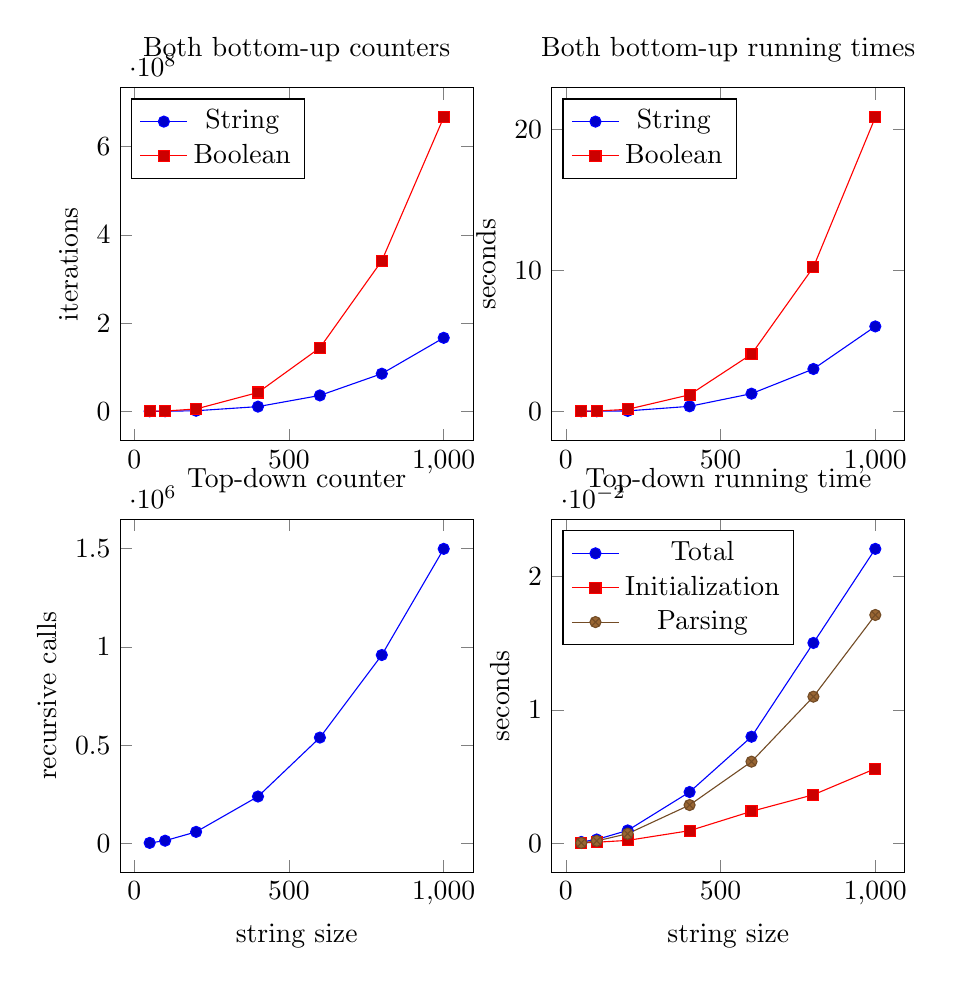
\begin{tikzpicture}
    \begin{groupplot}[group style={group size=2 by 2},height=0.5\textwidth,width=0.5\textwidth] 
    \nextgroupplot[title=Both bottom-up counters, ylabel=iterations, legend pos=north west]
    \addplot coordinates {
        (50, 21121)
        (100, 167246)
        (200, 1334496)
        (400, 10668996)
        (600, 36003496)
        (800, 85337996)
        (1000, 166672496)};
    \addlegendentry{String}
    \addplot coordinates {
        (50, 83400)
        (100, 666800)
        (200, 5333600)
        (400, 42667200)
        (600, 144000800)
        (800, 341334400)
        (1000, 666668000)};
    \addlegendentry{Boolean}
    \nextgroupplot[title=Both bottom-up running times, ylabel=seconds, legend pos=north west]
    \addplot coordinates {
        (50, 0.000571)
        (100, 0.003931)
        (200, 0.031064)
        (400, 0.354137)
        (600, 1.25128)
        (800, 3.00095)
        (1000, 6.0186)};
    \addlegendentry{String}
    \addplot coordinates {
        (50, 0.002598)
        (100, 0.019514)
        (200, 0.142831)
        (400, 1.17313)
        (600, 4.05125)
        (800, 10.2203)
        (1000, 20.8444)};
    \addlegendentry{Boolean}
    \nextgroupplot[title=Top-down counter, xlabel=string size, ylabel=recursive calls]
    \addplot coordinates {
        (50, 3676)
        (100, 14851)
        (200, 59701)
        (400, 239401)
        (600, 539101)
        (800, 958801)
        (1000, 1498501)};
    \nextgroupplot[title=Top-down running time, xlabel=string size, ylabel=seconds, legend pos=north west]
    \addplot coordinates {
        (50, 0.000117)
        (100, 0.000302)
        (200, 0.000982)
        (400, 0.003857)
        (600, 0.007999)
        (800, 0.015024)
        (1000, 0.022071)};
    \addlegendentry{Total}
    \addplot coordinates {
        (50, 0.000048)
        (100, 0.000097)
        (200, 0.000234)
        (400, 0.000962)
        (600, 0.00241)
        (800, 0.003652)
        (1000, 0.005607)};
    \addlegendentry{Initialization}
    \addplot coordinates {
        (50, 0.000046)
        (100, 0.000195)
        (200, 0.000733)
        (400, 0.002882)
        (600, 0.006131)
        (800, 0.011)
        (1000, 0.017119)};
    \addlegendentry{Parsing}
    \end{groupplot}
\end{tikzpicture}
\caption{Both bottom-up and top-down parsers behaviours, grammar 1, case 1}
\end{figure}
\FloatBarrier

The `boolean' bottom-up parser follows exactly the predicted behaviour, the number of iterations going up following the equation \ref{eq:bottom-up_iterations} and its running time follows exactly the same curve since for each iteration the parser does exactly the same amount of loops.
For this grammar it is slower than the `string' version.

Here the top-down parser is faster than both bottom-up parsers.
To get a more precise result the initialization and the parsing process have been timed apart from each other.
We can see that the initialization time scales up a power function.
The parsing time seems to follow the curve of the recursive calls counter.
\\
\\
It is very easy to check the complexity of the two bottom-up parsers here by resolving for both an equation of the form $y = a \cdot x^3$ by replacing $x$ and $y$ by the coordinates of a point of their graphs.

Those are respectively the theorical expressions of the `boolean' and `string' bottom-up parsers:

\begin{align*}
    &y = 2.0844 \cdot 10^{-8} \cdot x^3 &y = 6.0186 \cdot 10^{-9} \cdot x^3
\end{align*}

\FloatBarrier
\begin{figure}[h]
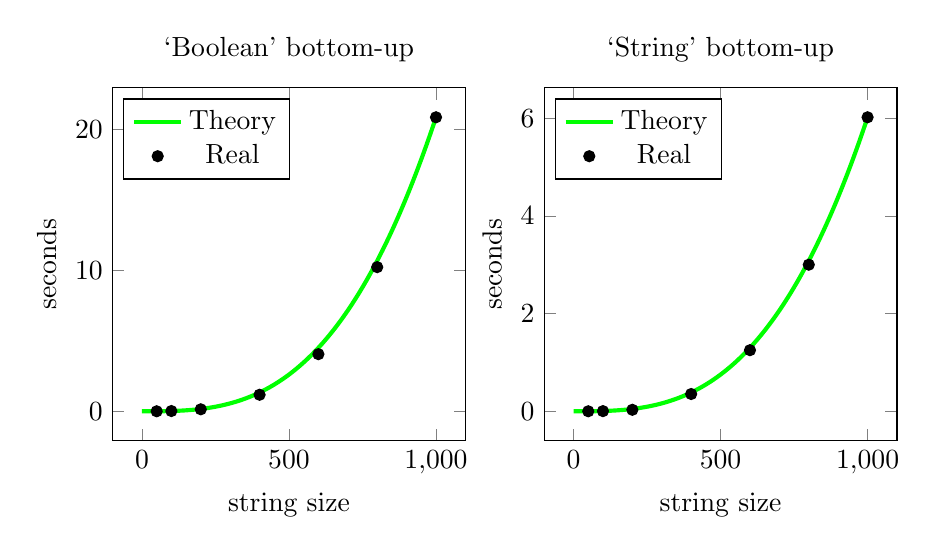
\begin{tikzpicture}
    \begin{groupplot}[group style={group size=2 by 1},height=0.5\textwidth,width=0.5\textwidth] 
    \nextgroupplot[title=`Boolean' bottom-up, xlabel=string size, ylabel=seconds, legend pos=north west]
    \addplot[domain=0:1000, samples=100, line width=1.5pt, green] {2.0844*(10^(-8))*(x^3)};
    \addlegendentry{Theory}
    \addplot[only marks, mark=*, mark size=2pt] coordinates {
        (50, 0.002598)
        (100, 0.019514)
        (200, 0.142831)
        (400, 1.17313)
        (600, 4.05125)
        (800, 10.2203)
        (1000, 20.8444)};
    \addlegendentry{Real}
    \nextgroupplot[title=`String' bottom-up, xlabel=string size, ylabel=seconds, legend pos=north west]
    \addplot[domain=0:1000, samples=100, line width=1.5pt, green] {6.0186*(10^(-9))*(x^3)};
    \addlegendentry{Theory}
    \addplot[only marks, mark=*, mark size=2pt] coordinates {
        (50, 0.000571)
        (100, 0.003931)
        (200, 0.031064)
        (400, 0.354137)
        (600, 1.25128)
        (800, 3.00095)
        (1000, 6.0186)};
    \addlegendentry{Real}
    \end{groupplot}
\end{tikzpicture}
\caption{Checking theorical fit, both bottom-up parsers}
\end{figure}
\FloatBarrier

The two functions fit almost perfectly to the points which confirms the $O(n^3)$ complexity for both bottom-up parsers.
\\
\\
The naive parser is very slow with that grammar, but it is possible to check its complexity too by resolving the equation $y = a \cdot 3^x$.

\begin{align*}
    &y = 2.146422 \cdot 10^{-10} \cdot 3^x
\end{align*}

\FloatBarrier
\begin{figure}[h]
\centering
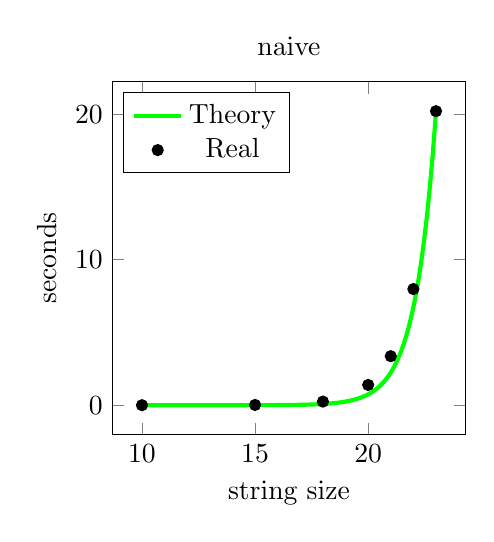
\begin{tikzpicture}
    \begin{groupplot}[group style={group size=1 by 1},height=0.5\textwidth,width=0.5\textwidth] 
    \nextgroupplot[title=naive, xlabel=string size, ylabel=seconds, legend pos=north west]
    \addplot[domain=10:23, samples=100, line width=1.5pt, green] {2.146422*(10^(-10))*(3^x)};
    \addlegendentry{Theory}
    \addplot[only marks, mark=*, mark size=2pt] coordinates {
        (10, 0.000236)
        (15, 0.017009)
        (18, 0.248498)
        (20, 1.39282)
        (21, 3.36746)
        (22, 7.98121)
        (23, 20.2071)};
    \addlegendentry{Real}
    \end{groupplot}
\end{tikzpicture}
\caption{Checking theorical fit, naive parser}
\end{figure}
\FloatBarrier

The theorical curve fits perfectly the running time of the naive parser which proves that the complexity of the naive parser is $O(3^n)$, it also shows that with that grammar this parser is very bad compared to the others.
\\
\\
The second pattern is the pattern only constituated by left parentheses: `$(\string^ n$', what makes it interesting is the fact that it is the worst case that we can generate with this grammar for the top-down parser.
The bottom-up parsers results will not be displayed in that case since they have the same behaviour as with the first case.

\FloatBarrier
\begin{figure}[h]
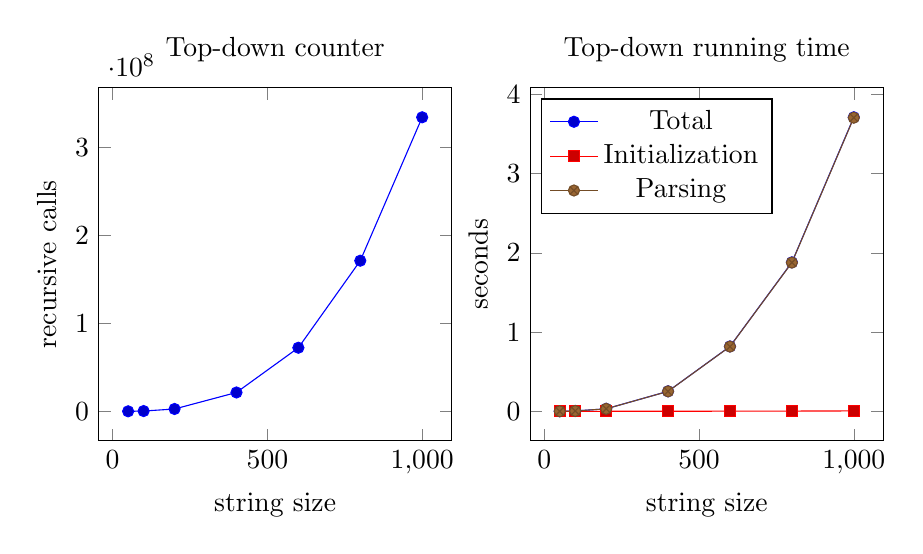
\begin{tikzpicture}
    \begin{groupplot}[group style={group size=2 by 1},height=0.5\textwidth,width=0.5\textwidth] 
    \nextgroupplot[title=Top-down counter, xlabel=string size, ylabel=recursive calls]
    \addplot coordinates {
        (50, 43526)
        (100, 340801)
        (200, 2696601)
        (400, 21453201)
        (600, 72269801)
        (800, 171146401)
        (1000, 334083001)};
    \nextgroupplot[title=Top-down running time, xlabel=string size, ylabel=seconds, legend pos=north west]
    \addplot coordinates {
        (50, 0.000605)
        (100, 0.004426)
        (200, 0.031748)
        (400, 0.252762)
        (600, 0.819545)
        (800, 1.88128)
        (1000, 3.71316)};
    \addlegendentry{Total}
    \addplot coordinates {
        (50, 0.000033)
        (100, 0.000119)
        (200, 0.000244)
        (400, 0.00081)
        (600, 0.001904)
        (800, 0.003088)
        (1000, 0.005164)};
    \addlegendentry{Initialization}
    \addplot coordinates {
        (50, 0.000561)
        (100, 0.004297)
        (200, 0.031488)
        (400, 0.251933)
        (600, 0.817614)
        (800, 1.87816)
        (1000, 3.70797)};
    \addlegendentry{Parsing}
    \end{groupplot}
\end{tikzpicture}
\caption{Top-down parser behaviour, grammar 1, case 2}
\end{figure}
\FloatBarrier

As we can see on the graph above in that case the initialization time of the top-down parser is negligible, the parsing time is the one that matters.
The parsing time follows exactly the same curve as the number of recursive calls.
Despite the fact that this case is the worst one for the top-down parser its running time remains lower than the other parsers.

We can conclude that for this grammar the top-down parser is more efficient than both bottom-up algorithms.
\\
\\
Here we can verify the complexity of the top-down parser by resolving the same equation as for the two bottom-up parsers.

\begin{align*}
    &y = 3.10797 \cdot 10^{-9} \cdot x^3
\end{align*}

\FloatBarrier
\begin{figure}[h]
\centering
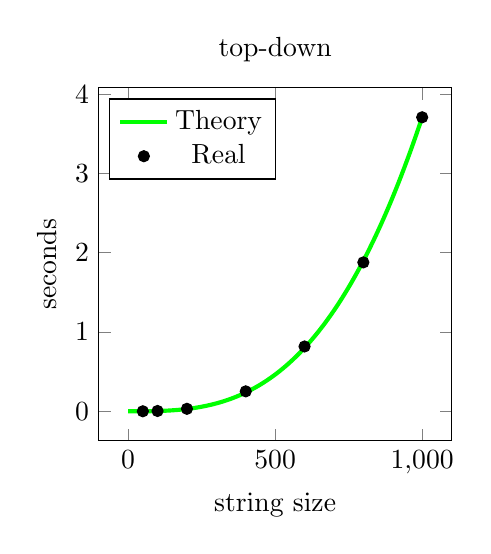
\begin{tikzpicture}
    \begin{groupplot}[group style={group size=1 by 1},height=0.5\textwidth,width=0.5\textwidth] 
    \nextgroupplot[title=top-down, xlabel=string size, ylabel=seconds, legend pos=north west]
    \addplot[domain=0:1000, samples=100, line width=1.5pt, green] {3.70797*(10^(-9))*(x^3)};
    \addlegendentry{Theory}
    \addplot[only marks, mark=*, mark size=2pt] coordinates {
        (50, 0.000561)
        (100, 0.004297)
        (200, 0.031488)
        (400, 0.251933)
        (600, 0.817614)
        (800, 1.87816)
        (1000, 3.70797)};
    \addlegendentry{Real}
    \end{groupplot}
\end{tikzpicture}
\caption{Checking theorical fit, grammar 1, case 2}
\end{figure}
\FloatBarrier

The curve fits perfectly the points of the top-down parser which proves that the complexity of the algorithm is $O(n^3)$.



\subsection{String starting with an `a'}
The grammar used in this section is the following:

\begin{align*} 
    &S \to AB\\
    &A \to a\\
    &B \to BB|a|b\\
\end{align*}

This grammar matches every string that begins with an `a', no matter what comes next.

\subsubsection{Number of iterations/recusive calls for each parser}

It is very interesting because with this grammar the top-down algorithm never uses the stored values in its table, no matter the pattern used.
At first one could think that this is a very bad thing, indeed since the top-down without the table is exactly the same as the naive parser it means that using this grammar they will both have the same behaviour.
But what is interesting is that the naive parser with this grammar and a string of size $n$ reacts like so:
$$
recursive \text{ } calls = 
\begin{cases}
    2n - 1 &\text{if string matches the grammar}\\
    n &\text{otherwise}
\end{cases}
$$

It is very easy to demonstrate those two results:
\begin{enumerate}
    \item In every pattern that does start with an `a' the number of recursive calls is $2n - 1$ because:
        \begin{itemize}
            \item[$-$] The initial call is $parse(S, 0, n)$.
            \item[$-$] The function will the recursively call $parse(A, 0, 1)$, which will return true since the \textit{terminal} `a' is equal to the character 0 of the string which is also `a'.
            \item[$-$] Then the function will call a second time $parse(B, 1, n)$.
            \item[$-$] That function will call $parse(B, 1, 2)$. That will return true no matter the character since `B' possesses both \textit{terminals} `a' and `b'.
            \item[$-$] Then it will call $parse(B, 2, n)$. This will repeat itself until $parse(B, n - 1, n)$ is called. At that moment it will return true.
            \item[$-$] At that moment the number of recursive calls is $(n - 1) * 2$ plus the initial call $1$, for a total of $2n - 1$ recursive calls. Note that every 2 steps this algorithm goes 1 step deeper into the recursive stack, this is an important fact for the experimentations.
        \end{itemize}
    \item In every pattern that does not start with an `a' the number of recursive calls is the size of the string $n$ because:
        \begin{itemize}
            \item[$-$] The initial call is $parse(S, 0, n)$. That function will enter in a loop for k going from $1$ to $n - 1$.
            \item[$-$] The function will then recursively call $parse(A, 0, 1)$, which returns false since the \textit{terminal} `a' is not equal to the character 0 of the string, which is `b'.
            \item[$-$] Then the function will call $parse(A, 0, k)$ until the end of the for loop. The calls will return false each time since `A' does not possess any \textit{non-terminals} rules.
            \item[$-$] So there is $1$ call plus $n - 1$ calls made by the first called function, for a total of $n$ recursive calls. Note that all the sub calls are made by the first called function, which limits the maximum reached recursive depth to only 2, it will be interesting to see in the experimentations how that has a very important impact.
        \end{itemize}
\end{enumerate}

With a behaviour like this one the naive parser is very efficient with that grammar.
Also in this section only the naive parser and both bottom-up parsers will be considered, since the naive and top-down one are the same.

With this grammar the best and worst case scenarios for the `string' bottom-up parser are:
\begin{itemize}
    \item[$-$] The worst case is a string following this pattern: `$b\string^ n$'.
    \item[$-$] The best case is a string following this pattern: `$a\string^ n$'.
    \item[$-$] Every case that is a mix between `a's and `b's will have a running time situated between the best and worst case.
        The more `b's there is in the string the closer the running time will be from the worst case and conversely with `a's.
\end{itemize}

It is now poosible to compare the anticipated behaviours of the `boolean' bottom-up and the naive parser, in both cases, using the function \ref{eq:bottom-up_iterations} and the two expressions from above.

\FloatBarrier
\begin{figure}[h]
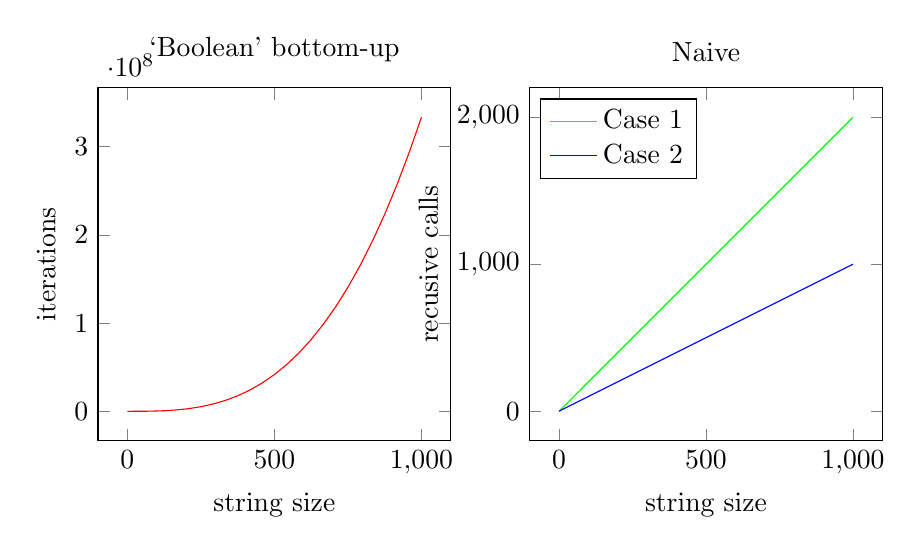
\begin{tikzpicture}
\begin{groupplot}[group style={group size=2 by 1},height=0.5\textwidth,width=0.5\textwidth, domain=0:1000]
\nextgroupplot[title=`Boolean' bottom-up, xlabel=string size, ylabel=iterations]
\addplot[red]{3 * x + ((2 / 6) * ((3 * (x^2) * (x + 1)) - (x * (x + 1) * ((2 * x) + 1))))};
\nextgroupplot[title=Naive, legend pos=north west,xlabel=string size, ylabel=recusive calls]
\addplot[green]{2 * x - 1};
\addlegendentry{Case 1}
\addplot[blue]{x};
\addlegendentry{Case 2}
\end{groupplot}
\end{tikzpicture}
\caption{Anticipation of the behaviours of the parsers, grammar 2}
\end{figure}
\FloatBarrier

Since the number of recursive calls of the naive parser with that grammar is linear it should be very effective compared to the `boolean' bottom-up one.
The naive parser should also be more effective than the `string' bottom-up parser since this one also follows a power function.

\subsubsection{Comparing the efficiency}

With that grammar there is only two cases to compare, the case in which the string matches the grammar and the case when it doesn't, except for the `string' bottom-up which has a behaviour depending on the pattern but for which those two patterns are the extrem cases.

The first used pattern is a case in which the strings match the grammar: `$a\string^ n$'.

\FloatBarrier
\begin{figure}[h]
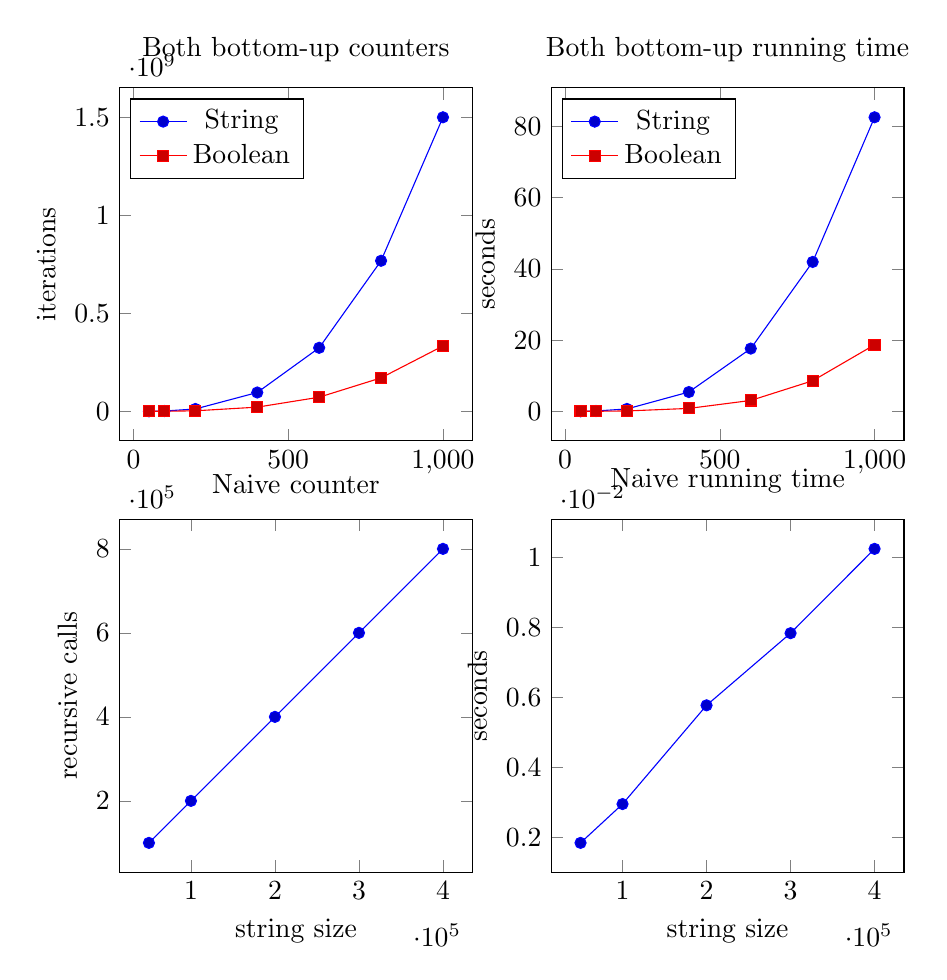
\begin{tikzpicture}
    \begin{groupplot}[group style={group size=2 by 2},height=0.5\textwidth,width=0.5\textwidth] 
    \nextgroupplot[title=Both bottom-up counters, ylabel=iterations, legend pos = north west]
    \addplot coordinates {
        (50, 187575)
        (100, 1500150)
        (200, 12000300)
        (400, 96000600)
        (600, 324000900)
        (800, 768001200)
        (1000, 1500001500)};
    \addlegendentry{String}
    \addplot coordinates {
        (50, 41800)
        (100, 333600)
        (200, 2667200)
        (400, 21334400)
        (600, 72001600)
        (800, 170668800)
        (1000, 333336000)};
    \addlegendentry{Boolean}
    \nextgroupplot[title=Both bottom-up running time, legend pos = north west, ylabel=seconds]
    \addplot coordinates {
        (50, 0.011391)
        (100, 0.08719)
        (200, 0.668587)
        (400, 5.41536)
        (600, 17.6169)
        (800, 41.9493)
        (1000, 82.579)};
    \addlegendentry{String}
    \addplot coordinates {
        (50, 0.001673)
        (100, 0.011914)
        (200, 0.101755)
        (400, 0.816538)
        (600, 3.0517)
        (800, 8.58051)
        (1000, 18.6903)};
    \addlegendentry{Boolean}
    \nextgroupplot[title=Naive counter, xlabel=string size, ylabel=recursive calls]
    \addplot coordinates {
        (50000, 99999)
        (100000, 199999)
        (200000, 399999)
        (300000, 599999)
        (400000, 799999)};
    \nextgroupplot[title=Naive running time, xlabel=string size, ylabel=seconds]
    \addplot coordinates {
        (50000, 0.001854)
        (100000, 0.002961)
        (200000, 0.005776)
        (300000, 0.007833)
        (400000, 0.010237)};
    \end{groupplot}
\end{tikzpicture}
\caption{Both bottom-up and naive parsers behaviours, grammar 2, case 1}
\end{figure}
\FloatBarrier

The running time of the naive parser compared to the two bottom-up ones with this grammar is so small that it is needed to use different string sizes in order to get relevant results.

With this grammar and that case the `boolean' bottom-up parser is faster than the `string' version.

A limitation of the top-down parser is that it needs to allocate memory for its table, but with strings of the size that are used in this experimentation it is not possible to allocate the memory.
So even if the behaviour is theoricaly exactly the same as with the naive parser in practice with a classic computer it is not possible to parse strings that long with the top-down parser.

The running time of the naive parser is linear, which makes sense since its number of recursive calls is linear too.

An interesting thing is that even if the running time of the naive parser remains very small with big string sizes the maximum size of the recursive stack was reached for strings bigger than 410000 characters.
This can be explained by the fact that when the string size $n$ increases the algorithm goes deeper and deeper in the stack: 1 more level of depth every 2 recursive calls.
This is not an issue that we will be able to see with a pattern that does not starts with a `b', indeed in that case as explained in section 3.2.2.1, case 2, the maximum recursive depth accessed is 2, which will allow the parser to parse longer strings.

The second used pattern is a case in which the strings do not match the grammar: `$b\string^ n$'.

\FloatBarrier
\begin{figure}[h]
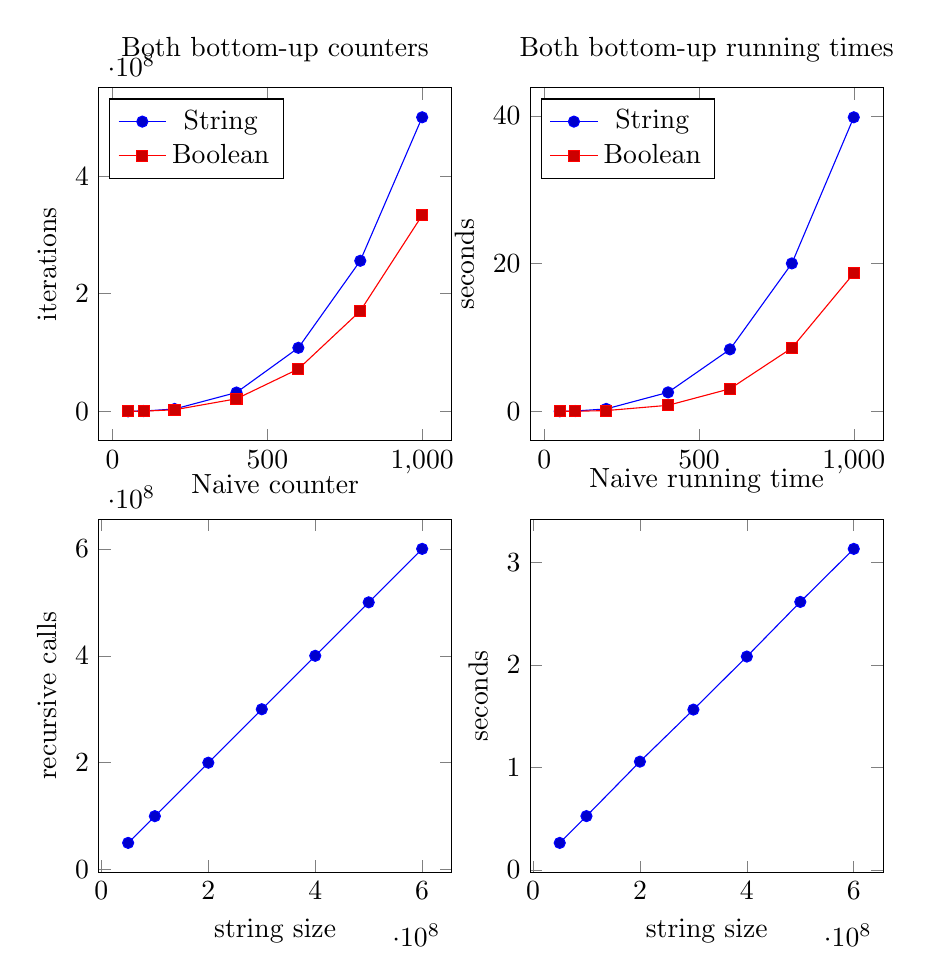
\begin{tikzpicture}
    \begin{groupplot}[group style={group size=2 by 2},height=0.5\textwidth,width=0.5\textwidth] 
    \nextgroupplot[title=Both bottom-up counters, ylabel=iterations, legend pos = north west]
    \addplot coordinates {
        (50, 62625)
        (100, 500250)
        (200, 4000500)
        (400, 32001000)
        (600, 108001500)
        (800, 256002000)
        (1000, 500002500)};
    \addlegendentry{String}
    \addplot coordinates {
        (50, 41800)
        (100, 333600)
        (200, 2667200)
        (400, 21334400)
        (600, 72001600)
        (800, 170668800)
        (1000, 333336000)};
    \addlegendentry{Boolean}
    \nextgroupplot[title=Both bottom-up running times, legend pos = north west, ylabel=seconds]
    \addplot coordinates {
        (50, 0.005147)
        (100, 0.043097)
        (200, 0.329631)
        (400, 2.56894)
        (600, 8.39397)
        (800, 20.0372)
        (1000, 39.8311)};
    \addlegendentry{String}
    \addplot coordinates {
        (50, 0.001673)
        (100, 0.011914)
        (200, 0.101755)
        (400, 0.816538)
        (600, 3.0517)
        (800, 8.58051)
        (1000, 18.6903)};
    \addlegendentry{Boolean}
    \nextgroupplot[title=Naive counter, xlabel=string size, ylabel=recursive calls]
    \addplot coordinates {
        (50000000, 50000000)
        (100000000, 100000000)
        (200000000, 200000000)
        (300000000, 300000000)
        (400000000, 400000000)
        (500000000, 500000000)
        (600000000, 600000000)};
    \nextgroupplot[title=Naive running time, xlabel=string size, ylabel=seconds]
    \addplot coordinates {
        (50000000, 0.262654)
        (100000000, 0.524298)
        (200000000, 1.05584)
        (300000000, 1.56371)
        (400000000, 2.08152)
        (500000000, 2.61476)
        (600000000, 3.13239)};
    \end{groupplot}
\end{tikzpicture}
\caption{Both bottom-up and naive parsers behaviour, grammar 2, case 2}
\end{figure}
\FloatBarrier

The curves of the `boolean' are the same as with the last case since no matter the pattern used that parser will always have the same behaviour with that grammar.
This case is the best case for the `string' bottom-up parser and the running time is indeed lower than with the first case, however it still takes more time than the `boolean' version.

With that case it was possible to parse a word of 600 millions character in about 3 seconds with the naive parser, which is very impressive.
The parser was maybe able to parse the word in some seconds but the longest part was in fact the time to generate the string and also the time to pass such string in parameter to some functions.
The running time is once again linear as expected.
\\
\\
With both the best and the worst case scenarios for the `string' bottom-up parser it is possible to display the area between the two curves.
The running time of that parser will always be contained in the blue area and the more `$b$'s there is in the given string the more the running time will follow a close curve from the worst case and conversely.

\FloatBarrier
\begin{figure}[h]
    \centering
    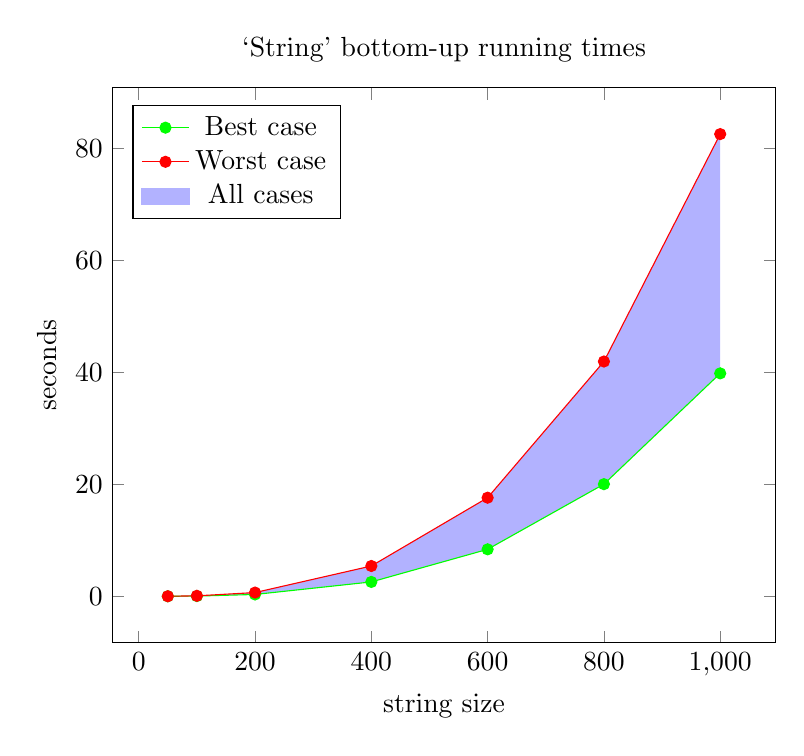
\begin{tikzpicture}
        \begin{axis}[title=`String' bottom-up running times, ylabel=seconds, xlabel=string size, legend pos = north west]
        \addplot[mark=*, green, name path=plot1] coordinates {
        (50, 0.005147)
        (100, 0.043097)
        (200, 0.329631)
        (400, 2.56894)
        (600, 8.39397)
        (800, 20.0372)
        (1000, 39.8311)};
        \addlegendentry{Best case}
        \addplot[mark=*, red, name path=plot2] coordinates {
        (50, 0.011391)
        (100, 0.08719)
        (200, 0.668587)
        (400, 5.41536)
        (600, 17.6169)
        (800, 41.9493)
        (1000, 82.579)};
        \addlegendentry{Worst case}
        \addplot[blue!30] fill between[of=plot1 and plot2];
        \addlegendentry{All cases}
        \end{axis}
    \end{tikzpicture}
    \caption{Running time of the `string' bottom-up parser, grammar 3}
\end{figure}
\FloatBarrier


\subsection{String ending with an `a'}
The grammar used in this section is the following:

\begin{align*}
    &S \to BA\\
    &A \to a\\
    &B \to BB|a|b
\end{align*}

\subsubsection{Number of iterations/recursive calls for each parser}

An interesting thing to notice is that with that grammar and a string of size $n$, no matter the used pattern, the amount of needed iterations or recursive calls will be the same for the naive, top-down and `boolean' bottom-up parsers.

The `string' bottom-up parser follows exactly the same behaviour as with the previous grammar.

By decomposing the behaviour of the naive parser one can find out that for any pattern it evolves following that sequence:
\begin{equation}\label{seq:naive}
n + (n - 1)^2
\end{equation}

It can be demonstrated like so:

\begin{itemize}
    \item[$-$] The initial call is $parse(S, 0, n)$
    \item[$-$] Then it calls $parse(B, 0, 1)$, which returns true no matter the character.
    \item[$-$] Then it calls $parse(A, 1, n)$, which returns false since A doesn't possess any \textit{non-terminals}.
    \item[$-$] Then it calls $parse(B, 0, 2)$, which returns true by doing 2 more recursive calls, $parse(B, 0, n)$ will always return true and do two more recursive calls each time it is called.
    \item[$-$] The process ends up when $parse(A, n - 1, n)$ is called, then it returns true or false depending on if the last character is an `a' or a `b'. No matter the result, and so the pattern, the algorithm will always make the same amount of recursive calls.
    \item[$-$] When it ends up the number of recursive calls is $1$ for the initial call, plus $n - 1$ for each time it has called parse(A, x, n), plus $(n - 1)^2$ for each time it has called parse(B, 0, x) and all the recursive calls it made. So the total number of recursive calls is $n + (n - 1)^2$ for the naive parser.
\end{itemize}

The top-down parser follows the exact same behaviour as the naive parser, to parse a string of size $n$ it will also need $n + (n - 1)^2$ recursive calls.

However some sub-problems will not need to be recomputed by the top-down parser, it is possible to show that, for a string of size $n$ and whatever pattern is used, it needs to solve that many sub-problems:
\begin{equation}\label{seq:top-down}
n + (n - 1)^2 - \dfrac{(n - 2) \cdot (n - 1)}{2}
\end{equation}

Here is the demonstration:

\begin{itemize}
    \item[$-$] The running process is exactly the same as for the naive one, the difference is that some results have already been computed and can be directly returned.
    \item[$-$] The amount of results already stored in the table and then asked again increases by one for each level of recursive depth when $parse(B, 0, x)$ is called.
    \item[$-$] This amount corresponds to a triangular number sequence: $\dfrac{n \cdot (n + 1)}{2}$. The formula needs to be twisted a little to match the string size $n$ and the number of asked already known results is $\dfrac{(n - 1) \cdot (n - 2)}{2}$.
    \item[$-$] Then the total amount of solved sub-problems is just the number of recursive calls minus the expression above: $n + (n - 1)^2 - \dfrac{(n - 2) \cdot (n - 1)}{2}$.
\end{itemize}

It is now possible to compare the anticipated behaviours of the naive, top-down and bottom-up parsers, using functions \ref{seq:naive} and \ref{eq:bottom-up_iterations}.

\FloatBarrier
\begin{figure}[h]
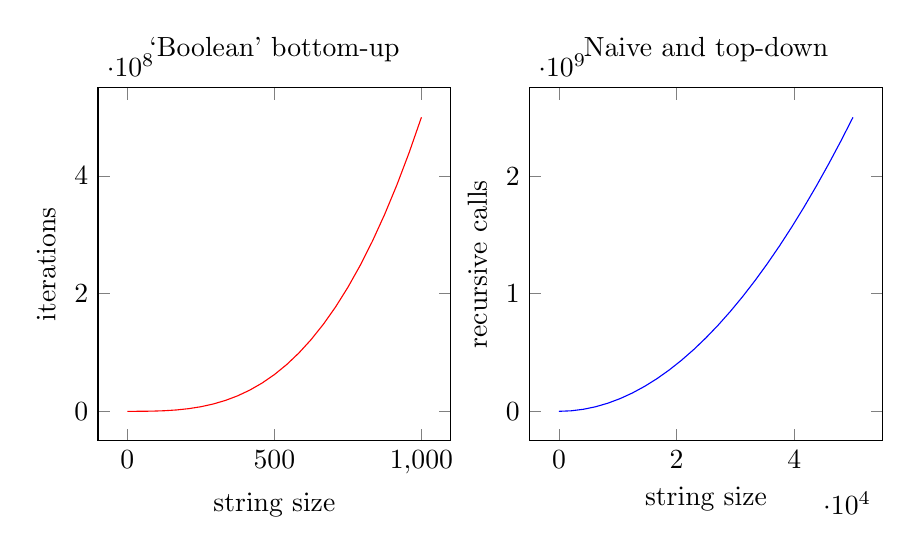
\begin{tikzpicture}
    \begin{groupplot}[group style={group size=2 by 1},height=0.5\textwidth,width=0.5\textwidth] 
    \nextgroupplot[title=`Boolean' bottom-up, xlabel=string size, ylabel=iterations]
    \addplot[red, domain=0:1000]{2 * x + ((3 / 6) * ((3 * (x^2) * (x + 1)) - (x * (x + 1) * ((2 * x) + 1))))};
    \nextgroupplot[title=Naive and top-down, xlabel=string size, ylabel=recursive calls]
    \addplot[blue, domain=0:50000]{x + (x - 1)^2};
    \end{groupplot}
\end{tikzpicture}
\caption{Anticipation of the behaviours of the parsers, grammar 3}
\end{figure}
\FloatBarrier

The `boolean' bottom-up parser follows a power function with an exponent of three as usual, but the top-down and naive parsers will follow a power function with an exponent of two with that grammar.

\subsubsection{Comparing the efficiency}

Except for the `string' bottom-up parser, with this grammar there is no particular cases, any pattern will be as long to parse as another by any of the three other parsers, the first used pattern is $a^n$.

\FloatBarrier
\begin{figure}[h]
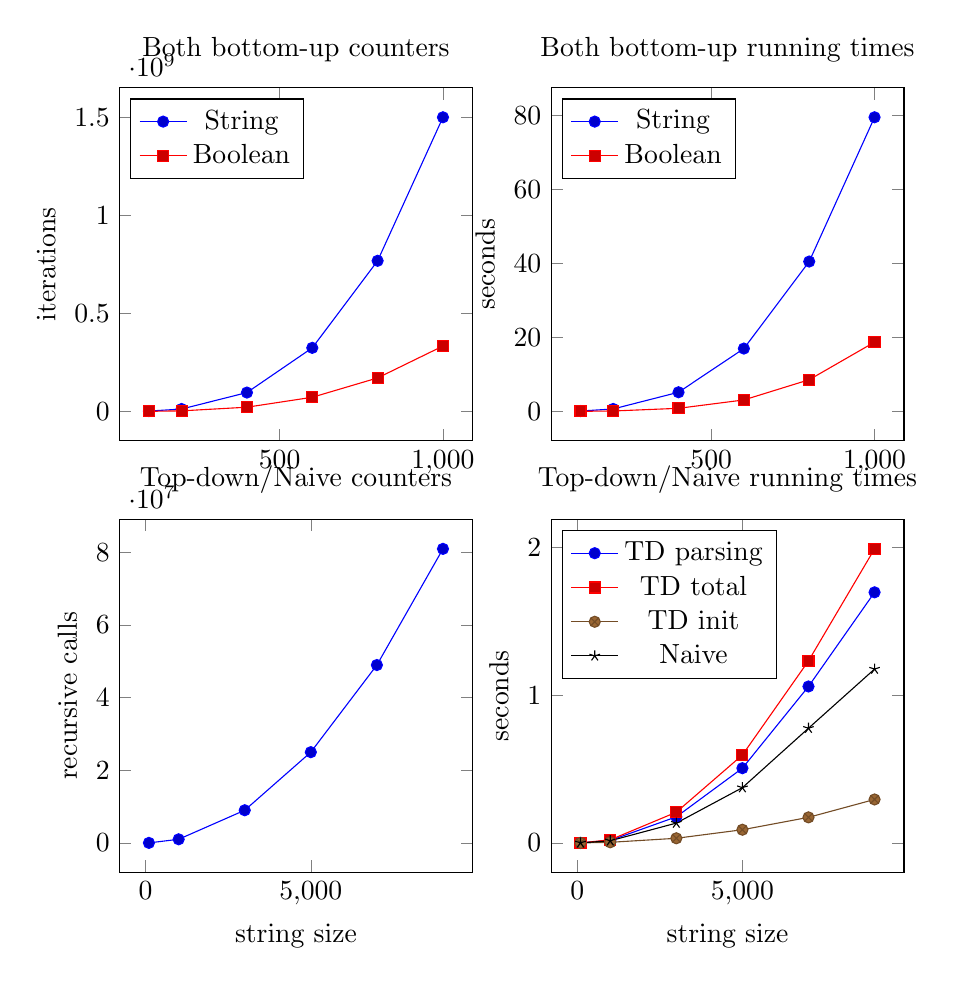
\begin{tikzpicture}
    \begin{groupplot}[group style={group size=2 by 2},height=0.5\textwidth,width=0.5\textwidth] 
    \nextgroupplot[title=Both bottom-up counters, ylabel=iterations, legend pos = north west]
    \addplot coordinates {
        (100, 1500150)
        (200, 12000300)
        (400, 96000600)
        (600, 324000900)
        (800, 768001200)
        (1000, 1500001500)};
    \addlegendentry{String}
    \addplot coordinates {
        (100, 333600)
        (200, 2667200)
        (400, 21334400)
        (600, 72001600)
        (800, 170668800)
        (1000, 333336000)};
    \addlegendentry{Boolean}
    \nextgroupplot[title=Both bottom-up running times, ylabel=seconds, legend pos = north west]
    \addplot coordinates {
        (100, 0.087481)
        (200, 0.652142)
        (400, 5.16778)
        (600, 16.9815)
        (800, 40.5165)
        (1000, 79.5284)};
    \addlegendentry{String}
    \addplot coordinates {
        (100, 0.012412)
        (200, 0.102093)
        (400, 0.82625)
        (600, 3.08987)
        (800, 8.56199)
        (1000, 18.7261)};
    \addlegendentry{Boolean}
    \nextgroupplot[title=Top-down/Naive counters, ylabel=recursive calls, xlabel=string size, legend pos = north west]
    \addplot coordinates {
        (100, 9901)
        (1000, 999001)
        (3000, 8997001)
        (5000, 24995001)
        (7000, 48993001)
        (9000, 80991001)};
    \nextgroupplot[title=Top-down/Naive running times, ylabel=seconds, legend pos=north west, xlabel=string size]
    \addplot coordinates {
        (100, 0.000158)
        (1000, 0.016837)
        (3000, 0.176553)
        (5000, 0.50593)
        (7000, 1.05917)
        (9000, 1.69652)};
    \addlegendentry{TD parsing}
    \addplot coordinates {
        (100, 0.00027)
        (1000, 0.020982)
        (3000, 0.207965)
        (5000, 0.595206)
        (7000, 1.23223)
        (9000, 1.99075)};
    \addlegendentry{TD total}
    \addplot coordinates {
        (100, 0.000091)
        (1000, 0.004109)
        (3000, 0.031383)
        (5000, 0.089245)
        (7000, 0.17303)
        (9000, 0.29419)};
    \addlegendentry{TD init}
    \addplot coordinates {
        (100, 0.000173)
        (1000, 0.01458)
        (3000, 0.134243)
        (5000, 0.374054)
        (7000, 0.776454)
        (9000, 1.17694)};
    \addlegendentry{Naive}
    \end{groupplot}
\end{tikzpicture}
\caption{The 4 parsers behaviours, grammar 3}
\end{figure}
\FloatBarrier

With strings of sizes greater than $9,000$ the top-down parser could not allocate the table so the used strings did not exceed that size.

The same string sizes are used for the top-down and naive parsers, it is possible to see on the graphs above that despite the fact that the naive parser and the top-down parsers need the same amount of recursive calls the naive parser has a lower running time.

The only parser that needs a various number of iterations is the `string' bottom-up parser, the pattern `$a\string^ n$' was as previously its worst case, its best case with that grammar is the pattern `$b\string^ n$' as previously.
It is not a suprise to find out that the `string' bottom-up parser is slower than the `boolean' version with that grammar, since it follows the same behaviour as before.

Next are the results obtained with the `string' bottom-up parser, using the last results for the `boolean' bottom-up parser as reference.

\FloatBarrier
\begin{figure}[h]
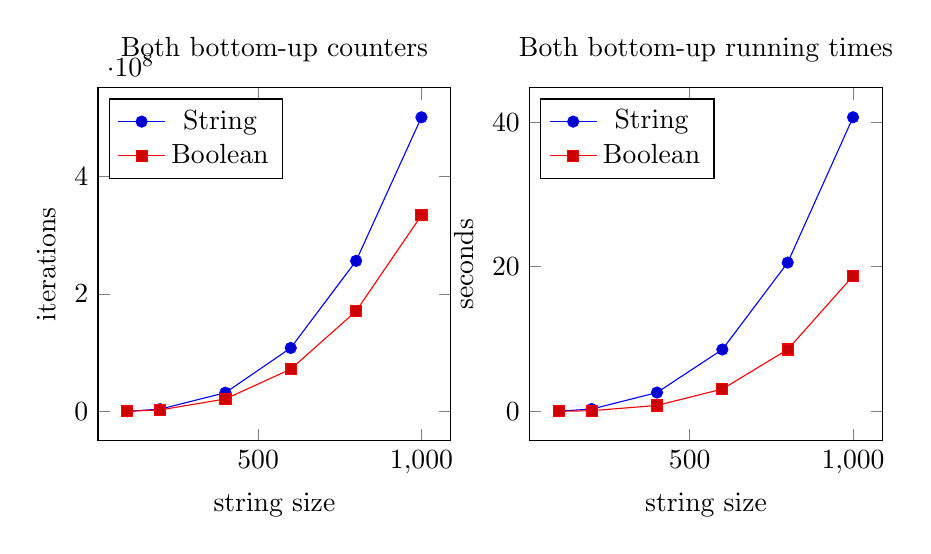
\begin{tikzpicture}
    \begin{groupplot}[group style={group size=2 by 1},height=0.5\textwidth,width=0.5\textwidth] 
    \nextgroupplot[title=Both bottom-up counters, ylabel=iterations, xlabel=string size, legend pos = north west]
    \addplot coordinates {
        (100, 500250)
        (200, 4000500)
        (400, 32001000)
        (600, 108001500)
        (800, 256002000)
        (1000, 500002500)};
    \addlegendentry{String}
    \addplot coordinates {
        (100, 333600)
        (200, 2667200)
        (400, 21334400)
        (600, 72001600)
        (800, 170668800)
        (1000, 333336000)};
    \addlegendentry{Boolean}
    \nextgroupplot[title=Both bottom-up running times, legend pos = north west, xlabel=string size, ylabel=seconds]
    \addplot coordinates {
        (100, 0.042859)
        (200, 0.322342)
        (400, 2.60902)
        (600, 8.56177)
        (800, 20.5762)
        (1000, 40.6679)};
    \addlegendentry{String}
    \addplot coordinates {
        (100, 0.012412)
        (200, 0.102093)
        (400, 0.82625)
        (600, 3.08987)
        (800, 8.56199)
        (1000, 18.7261)};
    \addlegendentry{Boolean}
    \end{groupplot}
\end{tikzpicture}
\caption{The `string' bottom-up parser worst case, grammar 3}
\end{figure}
\FloatBarrier

As with the previous grammar the best case of the `string' bottom-up parser is once again slower than the `boolean' version.
The running time follows exactly the same curve as the number of iterations for the `string' bottom-up parser.

It would be possible to plot the area containing all the possible cases of the `string' bottom-up parser once again but it would be the exact same figure as before since the running time of the parser for each pattern remains the same with both grammars.



\chapter{Linear grammar}

\section{Grammar preprocessing}

The goal was to implement an algorithm that would convert a context-free grammar into a grammar in the Chomsky normal-form, the most simple choice was to develop a new version of the Grammar class.

On its initialization the class is given a file that contains the grammar, which can be in any form.

The first thing that the class does is to replace all the \textit{non-terminal} variables by an index, starting at 0 for the \textit{start symbol} and increasing by 1 for every variable, the \textit{terminals} are also put in negative so there is no chance of confusion between the variables.

Then the grammar is converted to the Chomsky normal-form, following the same process as manually explained is section 1.1.2.

Finally the converted grammar is splitted into a set of \textit{terminal} rules and a set of \textit{non-terminal} rules.
\\
\\
The final grammar is stocked and can be accessed through the following variables:

\begin{itemize}
    \item[$-$] A 3D vector of integers named `non\_terminal\_rules'.
        \begin{enumerate}
            \item The first dimension represents the \textit{non-terminal} variable, converted as an index starting at 0 for the \textit{start symbol}.
            \item Each element of the second dimension is a right hand of the variable from the first dimension.
            \item The pairs of \textit{non-terminals} are stocked in the third dimension.
        \end{enumerate}
    \item[$-$] A 2D vector of integers named `terminal\_rules' that allows access to the \textit{terminal} rules.
    \item[$-$] Since there are no \textit{non-terminal} rules for every variable, when it is the case the variable is added to the string `nt\_variables'.
    \item[$-$] The string `t\_variables' is exactly the same as the one above but for the \textit{terminal} rules.
\end{itemize}

For example if one gives the following grammar to the program:

\begin{align*}
    &S \to Ac | b\\
    &A \to aS | aB\\
    &B \to bS\\
\end{align*}

This is how the grammar will be stocked:

\begin{itemize}
    \item[$-$] `non\_terminal\_rules' =
        \begin{align*}
            &0 \to 0\text{ }0 | 2\text{ }1 | 2\text{ }3 &2 \to\\
            &1 \to 0\text{ }3                           &3 \to\\
        \end{align*}
    \item[$-$] `terminal\_rules' =
        \begin{align*}
            &0 \to  &2 \to (\\
            &1 \to  &3 \to )\\
        \end{align*}
    \item[$-$] `nt\_variables' = "0 1"
    \item[$-$] `t\_variables' = "2 3"
\end{itemize}

The symbol `$|$' indicates the separation of the second dimension of the vector.
As we can see in the variables content above the \textit{non-terminals} are converted in indices.

That preprocessing allows one to give a linear grammar to the program without bothering to convert anything by advance.

Since the conversion of a linear grammar in the Chomsky normal-form often add new rules there is no reason to think that it could in any way fasten the parsing process to automaticly convert a linear grammar instead of directly giving the algorithm a Chomsky normal-form grammar.

\section{Implementation of a linear grammar parser}

Converting a grammar to the Chomsky normal-form cannot improve the running time of the parsers but a parser that directly parses strings using a linear grammar can be faster.

To implement a linear grammar parser the easiest choice was to use the actual top-down parser as basis for the new parser.
The program now contains a LinearGrammar class which simply stocks a linear grammar in the $rules$ variable without doing any modifications to the characters, the variable $non\_terminals$ is a string linking a \textit{non-terminal} to its index in the rules.
The parser is concived in such a way that it can parse a string using a linear grammar but also a grammar in the Chomsky normal-form.
Since the algorithm is based on the top-down parser if it is given a grammar in the Chomsky normal-form it will need the same number of resursive calls as the top-down parser would.

\FloatBarrier
\begin{algorithm}
\caption{Linear grammar parser}
\label{parse}
\begin{algorithmic}[1]
    \State $table$ is a 3d array of 0
    \State $s \gets input\_string$
    \Procedure{parse}{$var, i, j$} \Comment{Recursive parser function}
        \If{$table[var, i, j] != 0$}
            \State \textbf{return} $(table[var, i, j] == 1)$
        \EndIf
        \ForAll{$right\_hand \in rules[var]$}
            \If{$right\_hand.size() == j - i \land s.size() - i \geq j - i$}
                \State $bool \text{ } is\_equal \gets true$
                \For{$k \gets 0: k < right\_hand.size()$}
                    \If{$s[i + k] \neq right\_hand[k]$}
                       \State $is\_equal \gets false$
                        \State \textbf{break}
                    \EndIf
                \EndFor
                \If{$is\_equal$}
                    \State $table[var, i, j] \gets 1$
                    \State \textbf{return} $true$
                \EndIf
            \EndIf
            \State $var\_1, var\_2, var\_3 \text{ } are \text{ } characters$
            \If{$right\_hand.size() == 1$}
                \State $var\_1 \gets right\_hand[0]$
                \If{$var\_1 \geq \text{} 'A' \land var\_1 \leq\text{}'Z'$}
                    \If{$parse(non\_terminals.find(var\_1), i, j)$}
                        \State $table[var, i, j] \gets 1$
                        \State \textbf{return} $true$
                    \EndIf
                \EndIf
            \ElsIf{$j - i \geq 2 \land right\_hand.size() == 2$}
                \State $var\_1 \gets right\_hand[0]$
                \State $var\_2 \gets right\_hand[1]$
                \If{$var\_1 \geq \text{} 'A' \land var\_1 \leq \text{} 'Z' \land var\_2 \geq \text{} 'A' \land var\_2 \leq \text{} 'Z'$}
                    \For{$k \gets i + 1: k < j$}
                        \If{$parse(non\_terminals.find(var\_1), i, k) \land parse(non\_terminals.find(var\_2), k, j)$}
                            \State $table[var, i, j] \gets 1$
                            \State \textbf{return} $true$
                        \EndIf
                    \EndFor
                \ElsIf{$(var\_1 < \text{} 'A' \lor var\_1 > \text{} 'Z') \land var\_2 \geq \text{}'A' \land var\_2 \leq \text{} 'Z'$}
                    \If{$s[i] == var\_1$}
                        \If{$parse(non\_terminals.find(var\_2), i + 1, j)$}
                            \State $table[var, i, j] \gets 1$
                            \State \textbf{return} $true$
                        \EndIf
                    \EndIf
                    \algstore{part1}
\end{algorithmic}
\end{algorithm}
\FloatBarrier
\begin{algorithm}
\begin{algorithmic}[1]
                \algrestore{part1}
                \ElsIf{$var\_1 \geq \text{} 'A' \land var\_1 \leq \text{} 'Z' \land (var\_2 < \text{}'A' \lor var\_2 > \text{} 'Z')$}
                    \If{$s[j - 1] == var\_2$}
                        \If{$parse(non\_terminals.find(var\_1), i, j - 1)$}
                            \State $table[var, i, j] \gets 1$
                            \State \textbf{return} $true$
                        \EndIf
                    \EndIf
                \EndIf
            \ElsIf{$j - i \geq 3 \land right\_hand.size() == 3$}
                \State $var\_1 \gets right\_hand[0]$
                \State $var\_2 \gets right\_hand[1]$
                \State $var\_3 \gets right\_hand[2]$
                \If{$var\_1 \geq \text{} 'A' \land var\_1 \leq \text{} 'Z' \land (var\_2 < \text{}'A' \lor var\_2 > \text{} 'Z') \land var\_3 \geq \text{} 'A' \land var\_3 \leq \text{} 'Z'$}
                    \For{$k \gets i + 1; k < j - 1$}
                        \If{$parse(non\_terminals.find(var\_1), i, k) \land var\_2 == s[k] \land parse(non\_terminals.find(var\_3), k + 1, j)$}
                            \State $table[var, i, j] \gets 1$
                            \State \textbf{return} $true$
                        \EndIf
                    \EndFor
                \ElsIf{$(var\_1 < \text{} 'A' \lor var\_1 > \text{} 'Z') \land var\_2 \geq \text{}'A' \land var\_2 \leq \text{} 'Z') \land (var\_3 < \text{} 'A' \lor var\_3 > \text{} 'Z')$}
                    \If{$var\_1 == s[i] \land parse(non\_terminals.find(var\_2), i + 1, j - 1) \land var\_3 == s[j - 1]$}
                        \State $table[var, i, j] \gets 1$
                        \State \textbf{return} $true$
                    \EndIf
                \EndIf
            \EndIf
        \EndFor
        \State $table[var, i, j] \gets 2$
        \State \textbf{return} $false$
    \EndProcedure
\end{algorithmic}
\end{algorithm}
\FloatBarrier

Since this parser allows one to parse strings using a linear grammar instead of the Chomsky normal-form version it should be more efficient, indeed the linear grammar possesses less production rules and so the parser should need less recursive calls.

On the other hand since this parser is based on the same logic as the top-down parser its complexity is the same as that last one: $O(n^3)$.
That means that this parser will be more efficient in most practical cases but the same as the top-down parser in some other cases.

\section{Experimentation and comparison with previous parsers}

For this experimentation the first used linear grammar is the following.

\begin{align*}
    &S \to Ac | b\\
    &A \to aS | aB\\
    &B \to bS\\
\end{align*}

The linear parser is given the grammar above as it appears and the other parsers are given the automatically converted grammar as showed in section 4.1.

The used pattern to obtain the following results is `$a\string^ x \text{ } b \text{ } c\string^ x$', the strings generated by this pattern always match the grammar.

\FloatBarrier
\begin{figure}[h]
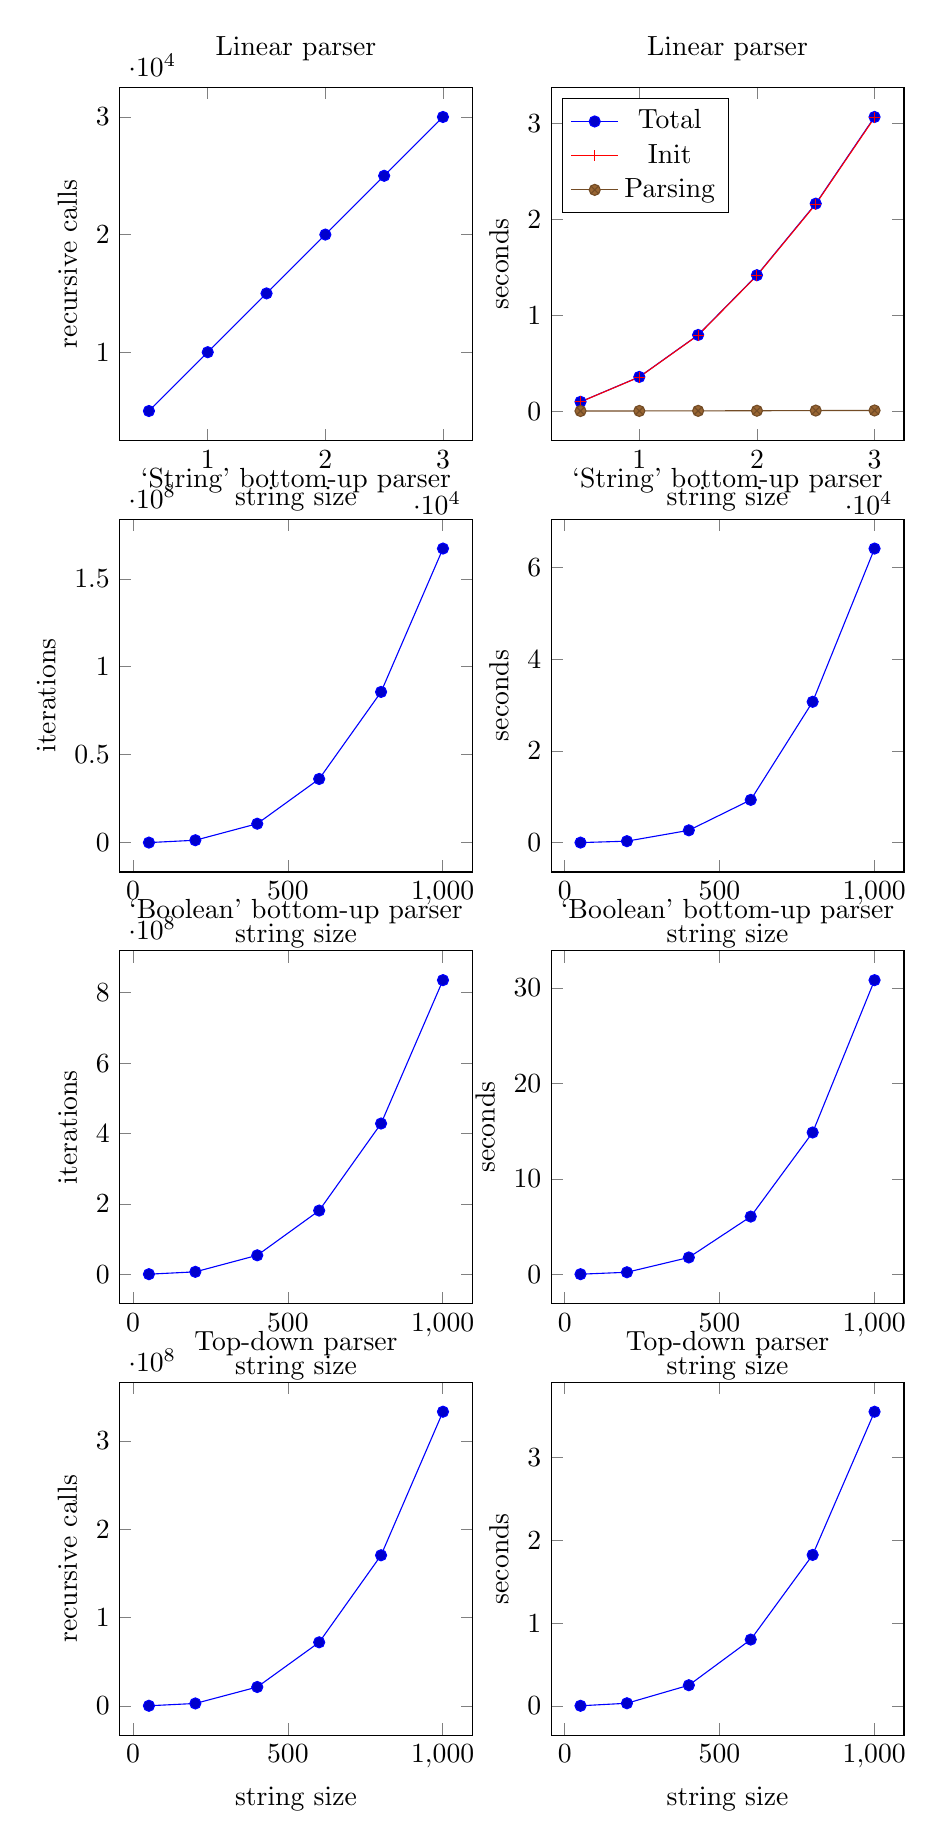
\begin{tikzpicture}
\begin{groupplot}[group style={group size=2 by 4},height=0.5\textwidth,width=0.5\textwidth]
    \nextgroupplot[title=Linear parser, xlabel=string size, ylabel=recursive calls, legend pos=north west]
    \addplot coordinates {
        (5001, 5001)
        (10001, 10001)
        (15001, 15001)
        (20001, 20001)
        (25001, 25001)
        (30001, 30001)};
    \nextgroupplot[title=Linear parser, xlabel=string size, ylabel=seconds, legend pos=north west]
    \addplot coordinates {
        (5001, 0.096865)
        (10001, 0.356474)
        (15001, 0.793719)
        (20001, 1.4169)
        (25001, 2.16269)
        (30001, 3.06646)};
    \addlegendentry{Total}
    \addplot[mark=+, red] coordinates {
        (5001, 0.095975)
        (10001, 0.354843)
        (15001, 0.791188)
        (20001, 1.41313)
        (25001, 2.15709)
        (30001, 3.05987)};
    \addlegendentry{Init}
    \addplot coordinates {
        (5001, 0.000854)
        (10001, 0.001589)
        (15001, 0.002483)
        (20001, 0.003718)
        (25001, 0.005531)
        (30001, 0.006541)};
    \addlegendentry{Parsing}
    \nextgroupplot[title=`String' bottom-up parser, xlabel=string size, ylabel=iterations, legend pos=north west]
    \addplot coordinates {
        (51, 23350)
        (201, 1358400)
        (401, 10756800)
        (601, 36195200)
        (801, 85673600)
        (1001, 167192000)};
    \nextgroupplot[title=`String' bottom-up parser, xlabel=string size, ylabel=seconds, legend pos=north west]
    \addplot coordinates {
        (51, 0.000608)
        (201, 0.031996)
        (401, 0.268441)
        (601, 0.932661)
        (801, 3.07346)
        (1001, 6.4173)};
    \nextgroupplot[title=`Boolean' bottom-up parser, xlabel=string size, ylabel=iterations, legend pos=north west]
    \addplot coordinates {
        (51, 110755)
        (201, 6768005)
        (401, 53736005)
        (601, 180904005)
        (801, 428272005)
        (1001, 835840005)};
    \nextgroupplot[title=`Boolean' bottom-up parser, xlabel=string size, ylabel=seconds, legend pos=north west]
    \addplot coordinates {
        (51, 0.003579)
        (201, 0.206125)
        (401, 1.75563)
        (601, 6.04026)
        (801, 14.8514)
        (1001, 30.8098)};
    \nextgroupplot[title=Top-down parser, xlabel=string size, ylabel=recursive calls, legend pos=north west]
    \addplot coordinates {
        (51, 41126)
        (201, 2657001)
        (401, 21294001)
        (601, 71911001)
        (801, 170508001)
        (1001, 333085001)};
    \nextgroupplot[title=Top-down parser, xlabel=string size, ylabel=seconds, legend pos=north west]
    \addplot coordinates {
        (51, 0.00054)
        (201, 0.031107)
        (401, 0.248966)
        (601, 0.801141)
        (801, 1.82474)
        (1001, 3.55611)};
\end{groupplot}
\end{tikzpicture}
\caption{Results with linear grammar 1, case 1}
\end{figure}
\FloatBarrier

The results above about the `String' and `boolean' bottom-up and top-down parsers are similar to results obtained before with various grammars.

Is is interesting to see that the linear parser needs $n$ recursive calls to parse a string of size $n$ which matches this grammar, the expected running time is expected to be linear too.
However the initialization process of the memoization table takes basicaly all the running time, the actual parsing time is too small to be relevant.
This shows a limitation of the linear parser in that case, the memoization table limits the input strings sizes that can be parsed.
Even with input strings bigger than $30000$ characters the parsing time is so low that even if it seems to follow a linear behaviour it is not relevant.

The next results are obtained using a set of strings that does not match the grammar, the pattern is `$a\string^ n$'.

The `boolean' bottom-up parser having the same behaviour for a given grammar the results are exactly the same for this pattern so they are not displayed.

\FloatBarrier
\begin{figure}[h]
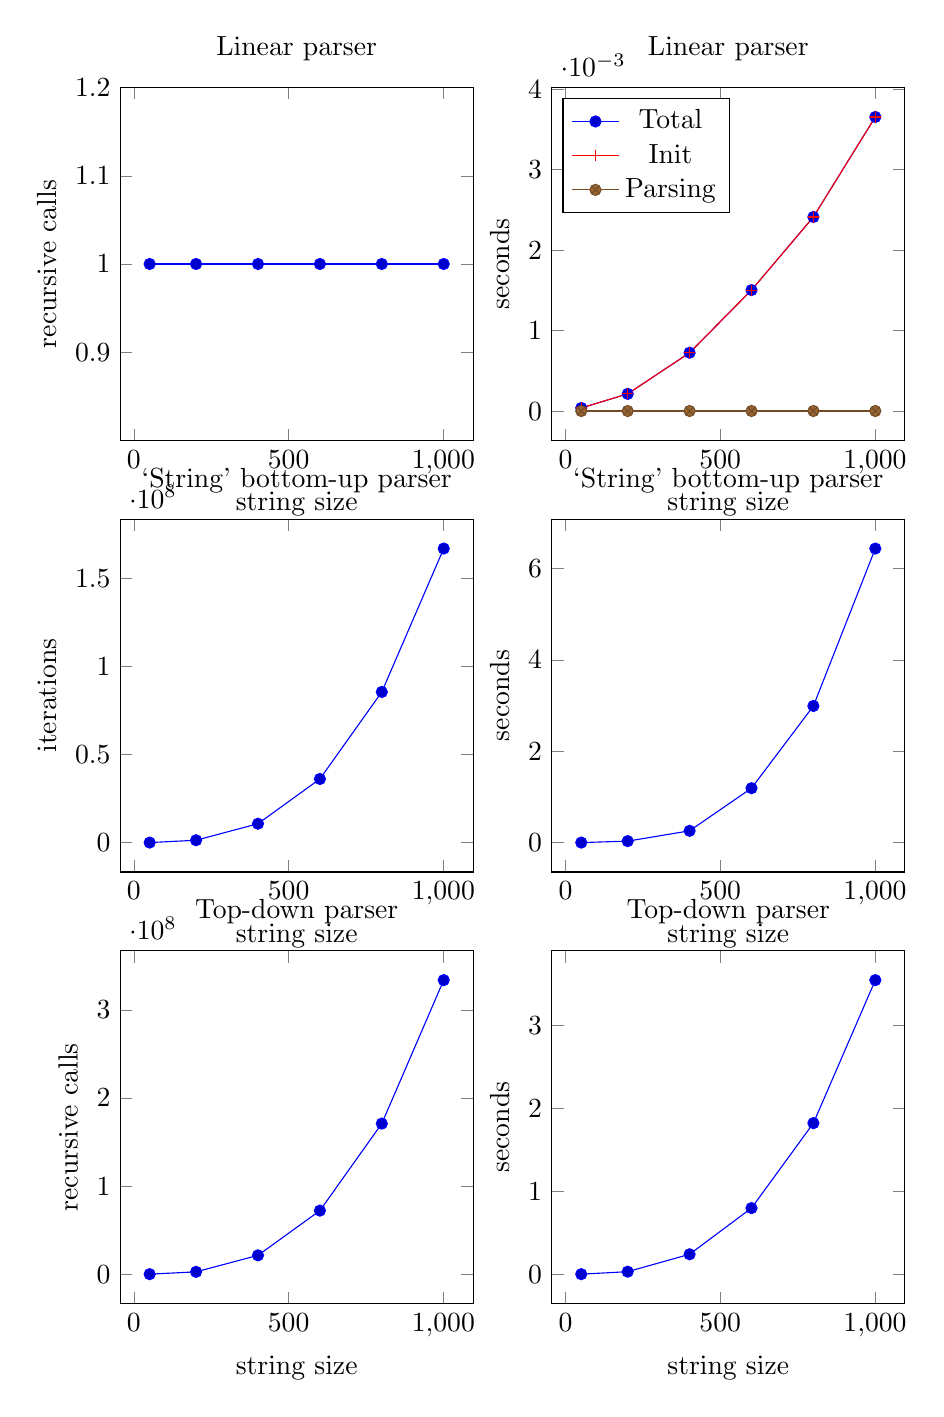
\begin{tikzpicture}
\begin{groupplot}[group style={group size=2 by 3},height=0.5\textwidth,width=0.5\textwidth]
    \nextgroupplot[title=Linear parser, xlabel=string size, ylabel=recursive calls, legend pos=north west]
    \addplot coordinates {
        (51, 1)
        (201, 1)
        (401, 1)
        (601, 1)
        (801, 1)
        (1001, 1)};
    \nextgroupplot[title=Linear parser, xlabel=string size, ylabel=seconds, legend pos=north west]
    \addplot coordinates {
        (51, 0.00004)
        (201, 0.000215)
        (401, 0.000726)
        (601, 0.001504)
        (801, 0.002412)
        (1001, 0.003654)};
    \addlegendentry{Total}
    \addplot[mark=+, red] coordinates {
        (51, 0.00004)
        (201, 0.000215)
        (401, 0.000726)
        (601, 0.001504)
        (801, 0.002412)
        (1001, 0.003654)};
    \addlegendentry{Init}
    \addplot coordinates {
        (51, 0.000002)
        (201, 0.000002)
        (401, 0.000002)
        (601, 0.000002)
        (801, 0.000002)
        (1001, 0.000002)};
    \addlegendentry{Parsing}
    \nextgroupplot[title=`String' bottom-up parser, xlabel=string size, ylabel=iterations, legend pos=north west]
    \addplot coordinates {
        (51, 22605)
        (201, 1355405)
        (401, 10750805)
        (601, 36186205)
        (801, 85661605)
        (1001, 167177005)};
    \nextgroupplot[title=`String' bottom-up parser, xlabel=string size, ylabel=seconds, legend pos=north west]
    \addplot coordinates {
        (51, 0.000547)
        (201, 0.032757)
        (401, 0.258234)
        (601, 1.19085)
        (801, 2.98934)
        (1001, 6.43343)};
    \nextgroupplot[title=Top-down parser, xlabel=string size, ylabel=recursive calls, legend pos=north west]
    \addplot coordinates {
        (51, 42951)
        (201, 2686801)
        (401, 21413601)
        (601, 72180401)
        (801, 170987201)
        (1001, 333834001)};
    \nextgroupplot[title=Top-down parser, xlabel=string size, ylabel=seconds, legend pos=north west]
    \addplot coordinates {
        (51, 0.000558)
        (201, 0.030692)
        (401, 0.240735)
        (601, 0.798035)
        (801, 1.8229)
        (1001, 3.54812)};
\end{groupplot}
\end{tikzpicture}
\caption{Results with linear grammar 1, case 2}
\end{figure}
\FloatBarrier

With this pattern the top-down needs a few more recursive calls than before, the change is so little that its running time is not touched by it.

With that pattern the number of recursive calls for the linear parser is always 1 since it just goes through the right-hands of `S' and then return false.
Once again the running time is high because of the initialization process, with that case the parsing time is constant and so small that it is not possible to represent it properly.

A limitation of the linear parser for this grammar in this form is the memoization table, indeed the parsing process is so short that it would be better to just use a naive version of this parser by not using the table.
This for two reason, the first obvious reason is that with this grammar the long part is to allocate the memory for the table.
The second reason is that once again with string longer than 40000 characters the used machine is not able to allocate enough memory for the table.

\subsection{Well balanced parentheses}

To really compare the efficiency of the linear parser with the other ones the best thing is to compare how they deal with the well balanced parenthese grammar.

The linear form of this grammar is the following.

\begin{align*}
    &S \to SS | (S) | ()
\end{align*}

The linear parser results will be compared with the top-down parser results in section 3.2.1.

With this grammar the linear parser behaves differently depending on the pattern of the strings.
The first considered case is the pattern `$)\string^ n$'.

\FloatBarrier
\begin{figure}[h]
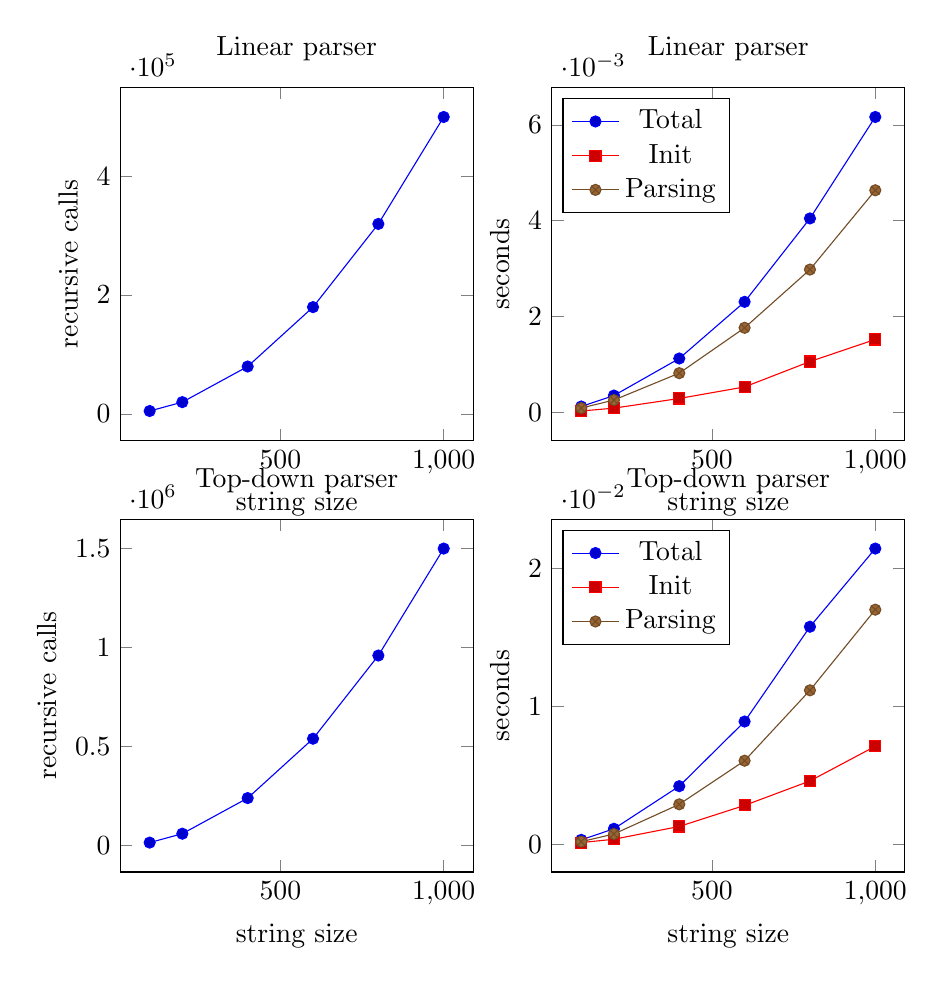
\begin{tikzpicture}
\begin{groupplot}[group style={group size=2 by 2},height=0.5\textwidth,width=0.5\textwidth]
    \nextgroupplot[title=Linear parser, xlabel=string size, ylabel=recursive calls, legend pos=north west]
    \addplot coordinates {
        (100, 4951)
        (200, 19901)
        (400, 79801)
        (600, 179701)
        (800, 319601)
        (1000, 499501)};
    \nextgroupplot[title=Linear parser, xlabel=string size, ylabel=seconds, legend pos=north west]
    \addplot coordinates {
        (100, 0.000117)
        (200, 0.000346)
        (400, 0.00112)
        (600, 0.002303)
        (800, 0.004045)
        (1000, 0.006164)};
    \addlegendentry{Total}
    \addplot coordinates {
        (100, 0.000023)
        (200, 0.000083)
        (400, 0.000285)
        (600, 0.000526)
        (800, 0.001056)
        (1000, 0.001518)};
    \addlegendentry{Init}
    \addplot coordinates {
        (100, 0.000085)
        (200, 0.000252)
        (400, 0.000814)
        (600, 0.001761)
        (800, 0.002977)
        (1000, 0.004633)};
    \addlegendentry{Parsing}
    \nextgroupplot[title=Top-down parser, xlabel=string size, ylabel=recursive calls, legend pos=north west]
    \addplot coordinates {
        (100, 14851)
        (200, 59701)
        (400, 239401)
        (600, 539101)
        (800, 958801)
        (1000, 1498501)};
    \nextgroupplot[title=Top-down parser, xlabel=string size, ylabel=seconds, legend pos=north west]
    \addplot coordinates {
        (100, 0.000317)
        (200, 0.00112)
        (400, 0.004209)
        (600, 0.008897)
        (800, 0.015769)
        (1000, 0.021436)};
    \addlegendentry{Total}
    \addplot coordinates {
        (100, 0.000119)
        (200, 0.000363)
        (400, 0.00129)
        (600, 0.002816)
        (800, 0.004587)
        (1000, 0.007104)};
    \addlegendentry{Init}
    \addplot coordinates {
        (100, 0.000188)
        (200, 0.000742)
        (400, 0.002894)
        (600, 0.006056)
        (800, 0.011159)
        (1000, 0.017006)};
    \addlegendentry{Parsing}
\end{groupplot}
\end{tikzpicture}
\caption{Results with linear grammar 2, case 1}
\end{figure}
\FloatBarrier

Here the two parsers running times follow the same behaviour as their number of recursive calls, the linear parser needs less recursive calls and so has a lower running time than the top-down parser.

For the second case the same parsers are used and the used pattern is `$(\string^ n$'.

\FloatBarrier
\begin{figure}[h]
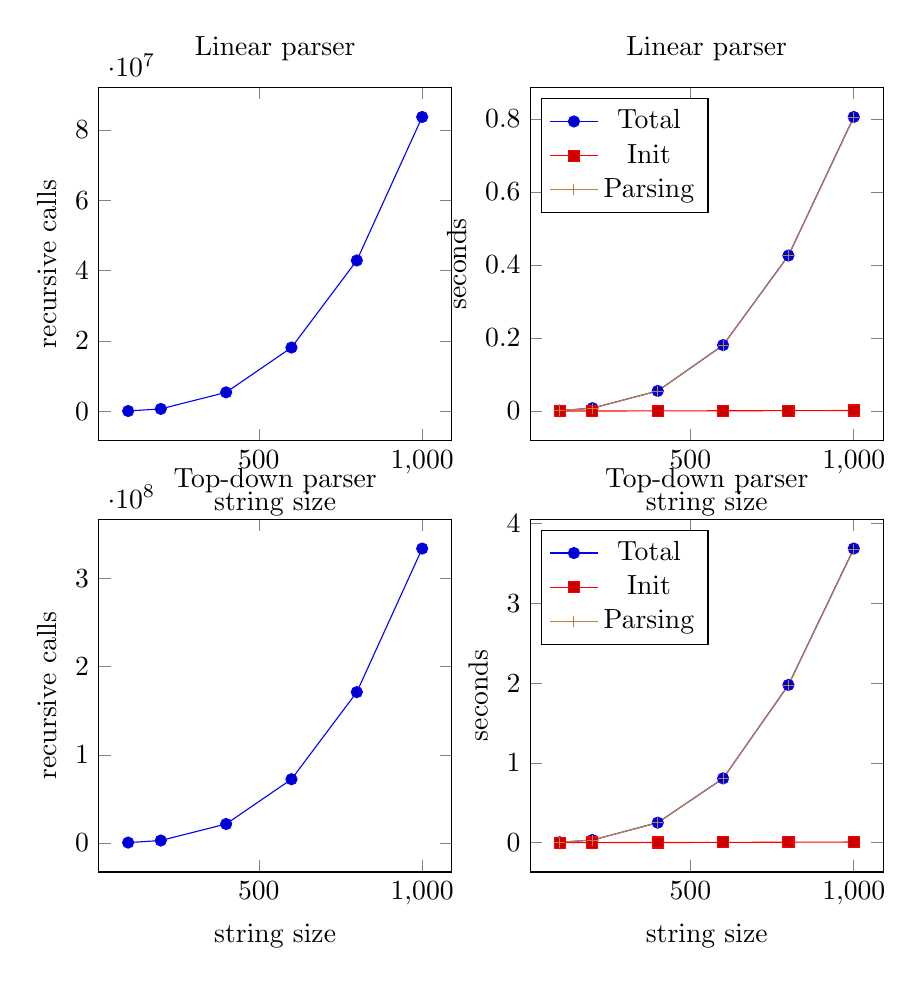
\begin{tikzpicture}
\begin{groupplot}[group style={group size=2 by 2},height=0.5\textwidth,width=0.5\textwidth]
    \nextgroupplot[title=Linear parser, xlabel=string size, ylabel=recursive calls, legend pos=north west]
    \addplot coordinates {
        (100, 87026)
        (200, 681551)
        (400, 5393101)
        (600, 18134651)
        (800, 42906201)
        (1000, 83707751)};
    \nextgroupplot[title=Linear parser, xlabel=string size, ylabel=seconds, legend pos=north west]
    \addplot coordinates {
        (100, 0.001216)
        (200, 0.007831)
        (400, 0.054993)
        (600, 0.180519)
        (800, 0.425874)
        (1000, 0.805482)};
    \addlegendentry{Total}
    \addplot coordinates {
        (100, 0.000031)
        (200, 0.000104)
        (400, 0.000292)
        (600, 0.00069)
        (800, 0.001011)
        (1000, 0.00142)};
    \addlegendentry{Init}
    \addplot[mark=+, brown] coordinates {
        (100, 0.001175)
        (200, 0.007718)
        (400, 0.054686)
        (600, 0.179794)
        (800, 0.42483)
        (1000, 0.804034)};
    \addlegendentry{Parsing}
    \nextgroupplot[title=Top-down parser, xlabel=string size, ylabel=recursive calls, legend pos=north west]
    \addplot coordinates {
        (100, 340801)
        (200, 2696601)
        (400, 21453201)
        (600, 72269801)
        (800, 171146401)
        (1000, 334083001)};
    \nextgroupplot[title=Top-down parser, xlabel=string size, ylabel=seconds, legend pos=north west]
    \addplot coordinates {
        (100, 0.004185)
        (200, 0.032133)
        (400, 0.25005)
        (600, 0.805403)
        (800, 1.97674)
        (1000, 3.68684)};
    \addlegendentry{Total}
    \addplot coordinates {
        (100, 0.000131)
        (200, 0.00039)
        (400, 0.001275)
        (600, 0.002598)
        (800, 0.005133)
        (1000, 0.0072)};
    \addlegendentry{Init}
    \addplot[mark=+, brown] coordinates {
        (100, 0.004044)
        (200, 0.031729)
        (400, 0.248752)
        (600, 0.802779)
        (800, 1.97158)
        (1000, 3.67961)};
    \addlegendentry{Parsing}
\end{groupplot}
\end{tikzpicture}
\caption{Results with linear grammar 2, case 2}
\end{figure}
\FloatBarrier

Here the initialization time is negligible before the parsing time for both parsers.

With that grammar the linear parser is more efficient than the top-down parser which was by far the most efficient compared to the other parser in section 3.2.1.

Here is the verification of the complexity of the linear parser.

\begin{align*}
    &y = 8.04034 \cdot 10^{-10} \cdot x^3
\end{align*}

\FloatBarrier
\begin{figure}[h]
\centering
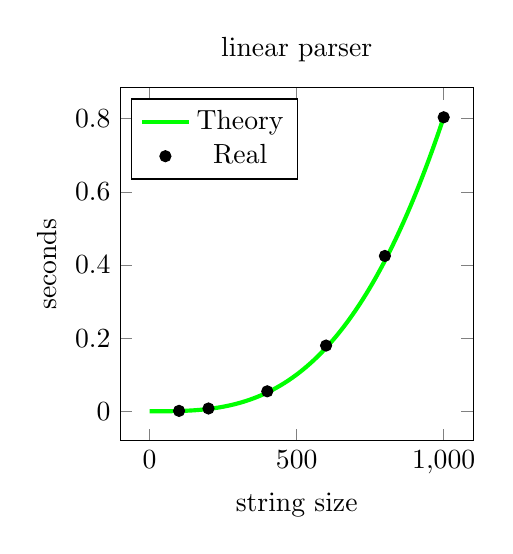
\begin{tikzpicture}
\begin{groupplot}[group style={group size=1 by 1},height=0.5\textwidth,width=0.5\textwidth]
    \nextgroupplot[title=linear parser, xlabel=string size, ylabel=seconds, legend pos=north west]
    \addplot[domain=0:1000, samples=100, line width=1.5pt, green] {8.04034*(10^(-10))*(x^3)};
    \addlegendentry{Theory}
    \addplot[only marks, mark=*, mark size=2pt] coordinates {
        (100, 0.001175)
        (200, 0.007718)
        (400, 0.054686)
        (600, 0.179794)
        (800, 0.42483)
        (1000, 0.804034)};
    \addlegendentry{Real}
\end{groupplot}
\end{tikzpicture}
\caption{Checking theorical fit, linear parser}
\end{figure}
\FloatBarrier

The real points fit perfectly the theorical curve which proves that the complexity of the linear parser really is $O(n^3)$.


\chapter{Error correction}
Since the corrections are directly effectued on the \textit{primitive symbols} the choice that seemed to be the simplest was to use the top-down parser as basis for the implementation of the error correction parser.

\section{Implementation of the character replacement}

The first step was to implement the character replacement, this is a modified version of the previous code of the top-down parser:

\FloatBarrier
\begin{algorithm}
    \caption{Top-down parser character modification}
    \label{parse}
    \begin{algorithmic}[1]
        \State $table$ is a 3d array of 0
        \State $s \gets input\_string$
        \Procedure{parse}{$var, i, j$} \Comment{Recursive parser function}
            \If{$table[var, i, j] != 0$}
                \State \textbf{return} $(table[var, i, j] == 1)$
            \EndIf
            \If{$i == j - 1$}
                \ForAll{$t \in terminal\_rule[var]$}
                    \If{$t == s[i]$}
                        \State $table[var, i, j] \gets \textcolor{red}{1}$
                        \State \textbf{return} \textcolor{red}{$table[var, i, j]$}
                    \EndIf
                \EndFor
                \textcolor{red}{\If{$terminal\_rule[var].size() > 0$}
                    \State $table[var, i, j] \gets 2$
                    \State \textbf{return} $table[var, i, j]$
                \EndIf}
            \Else
                \State \textcolor{red}{$min \gets INT\_MAX$}
                \ForAll{$nt \in non\_terminal\_rules[var]$}
                    \For{$k \gets i + 1; k < j$}
                        \State \textcolor{red}{$declare \text{ } res\_1 \text{ } and \text{ } res\_2$}
                        \textcolor{red}{\If{$(res\_1 \gets parse(nt[0], i, k)) < INT\_MAX \text{ } \land \text{ } (res\_2 \gets parse(nt[1], k, j)) < INT\_MAX$}
                            \If{$res\_1 + res\_2 - 1 < min$}
                                \State $min \gets res\_1 + res\_2 - 1$
                            \EndIf
                        \EndIf}
                    \EndFor
                \EndFor
                \State \textcolor{red}{$table[var, i, j] \gets min$}
                \State \textcolor{red}{\textbf{return} $table[var, i, j]$}
            \EndIf
            \State $table[var, i, j] \gets \textcolor{red}{INT\_MAX}$
            \State \textbf{return} \textcolor{red}{$table[var, i, j]$}
        \EndProcedure
    \end{algorithmic}
\end{algorithm}
\FloatBarrier

All the differences with the initial top-down parser are in red on this pseudo-code.

With those modifications the top-down parser now returns an integer when it parses a string:
\begin{itemize}
    \item[$-$] If the value is 1 it means that the string can be parsed without any modifications.
    \item[$-$] If the value is $x > 1$ it means that the string can be parsed with $x - 1$ modifications.
    \item[$-$] If the value is $INT\_MAX$, the maximum value of an integer, it means that the string cannot be parsed, no matter how much modifications could be made.
\end{itemize}

\section{Implementation of the character deletion}

Once the character modification is done the next step is to implement character deletion.

\FloatBarrier
\begin{algorithm}
    \caption{Top-down parser character deletion}
    \label{parse}
    \begin{algorithmic}[1]
        \State $table$ is a 3d array of 0
        \State $s \gets input\_string$
        \Procedure{parse}{$var, i, j$} \Comment{Recursive parser function}
            \If{$table[var, i, j] != 0$}
                \State \textbf{return} $(table[var, i, j] == 1)$
            \EndIf
            \If{$i == j - 1$}
                \ForAll{$t \in terminal\_rule[var]$}
                    \If{$t == s[i]$}
                        \State $table[var, i, j] \gets 1$
                        \State \textbf{return} $table[var, i, j]$
                    \EndIf
                \EndFor
                \If{$terminal\_rule[var].size() > 0$}
                    \State $table[var, i, j] \gets 2$
                    \State \textbf{return} $table[var, i, j]$
                \EndIf
            \Else
                \State $min \gets INT\_MAX$
                \State \textcolor{red}{$del\_1 \gets parse(var, i + 1, j)$}
                \State \textcolor{red}{$del\_2 \gets parse(var, i, j - 1)$}
                \ForAll{$nt \in non\_terminal\_rules[var]$}
                    \For{$k \gets i + 1; k < j$}
                        \State $declare \text{ } res\_1 \text{ } and \text{ } res\_2$
                        \If{\begin{varwidth}[t]{\linewidth}$(res\_1 \gets parse(nt[0], i, k)) < INT\_MAX \text{ } \land \text{ } (res\_2 \gets parse(nt[1], k, j)) < INT\_MAX$}\end{varwidth}
                            \If{$res\_1 + res\_2 - 1 < min$}
                                \State $min \gets res\_1 + res\_2 - 1$
                            \EndIf
                        \EndIf
                    \EndFor
                \EndFor
                \textcolor{red}{\If{$del\_2 < del\_1$}
                    \State $del\_1 \gets del\_2$
                \EndIf
                \If{$del\_1 < min$}
                    \State $min \gets del\_1$
                \EndIf}
                \State $table[var, i, j] \gets min$
                \State \textbf{return} $table[var, i, j]$
            \EndIf
            \State $table[var, i, j] \gets INT\_MAX$
            \State \textbf{return} $table[var, i, j]$
        \EndProcedure
    \end{algorithmic}
\end{algorithm}
\FloatBarrier

That algorithm returns the number of modifications plus deletions, the next step is to be able to return the corrected version of the input string.
Once such corrected string can be generated it will be trivial to know how much deletions and modifications were both needed.

\section{Recuperation of the corrected string}

In order to proceed to the recuperation of the corrected string a structure is used to contain the result of the parse function plus the corresponding corrected string.
The memoization table of the top-down parser will now contains datas of this structure.
The parse function will also now return a $parse\_result$ structure, it will also take the corrected string at its actual state as parameter.

This is is the pseudo-code with the modifications needed to be able to retrieve the corrected string.

\FloatBarrier
\begin{algorithm}
    \caption{Top-down parser correction and string recuperation}
    \label{parse}
    \begin{algorithmic}[1]
        \State $table$ is a 3d array of $parse\_result$
        \State $s \gets input\_string$
        \Procedure{parse}{$var, i, j, \textcolor{red}{sc}$} \Comment{Recursive parser function}
            \If{$table[var, i, j] != 0$}
                \State \textbf{return} $(table[var, i, j] == 1)$
            \EndIf
            \If{$i == j - 1$}
                \ForAll{$t \in terminal\_rule[var]$}
                    \If{$t == s[i]$}
                        \State \textcolor{red}{$table[var, i, j].result \gets 1$}
                        \State \textcolor{red}{$table[var, i, j].string \gets sc$}
                        \State \textbf{return} $table[var, i, j]$
                    \EndIf
                \EndFor
                \If{$terminal\_rule[var].size() > 0$}
                    \State \textcolor{red}{$table[var, i, j].result \gets 2$}
                    \State \textcolor{red}{$table[var, i, j].string \gets terminal\_rule[var][0]$}
                    \State \textbf{return} $table[var, i, j]$
                \EndIf
            \Else
                \State $min \gets INT\_MAX$
                \State \textcolor{red}{$new\_s \gets ""$}
                \State \textcolor{red}{$del\_1 \gets parse(var, i + 1, j, sc.substr(1, sc.size() - 1))$}
                \State \textcolor{red}{$del\_2 \gets parse(var, i, j - 1, sc.substr(0, sc.size() - 1))$}
                \ForAll{$nt \in non\_terminal\_rules[var]$}
                    \For{$k \gets i + 1; k < j$}
                        \State $res\_1 \gets parse(nt[0], i, k, \textcolor{red}{sc.substr(0, k - i)})$
                        \If{$res\_1\textcolor{red}{.result} < INT\_MAX$}
                            \State $res\_2 \gets parse(nt[1], k, j, \textcolor{red}{sc.substr(k - i, j - k)})$
                            \If{$res\_2\textcolor{red}{.result} < INT\_MAX$}
                                \If{$res\_1\textcolor{red}{.result} + res\_2\textcolor{red}{.result} - 1 < min$}
                                    \State $min \gets res\_1\textcolor{red}{.result} + res\_2\textcolor{red}{.result} - 1$
                                    \State \textcolor{red}{$new\_s \gets res\_1.string + res\_2.string$}
                                \EndIf
                            \EndIf
                        \EndIf
                    \EndFor
                \EndFor
                \State $table[var, i, j] \gets \textcolor{red}{min\_parse\_result(del\_1, del\_2, min, new\_string)}$
                \State \textbf{return} $table[var, i, j]$
            \EndIf
            \State \textcolor{red}{$table[var, i, j].result \gets INT\_MAX$}
            \State \textcolor{red}{$table[var, i, j].string \gets sc$}
            \State \textbf{return} $table[var, i, j]$
        \EndProcedure
    \end{algorithmic}
\end{algorithm}
\FloatBarrier

Such an algorithm will end by returning the corrected string plus the sum of all needed corrections and deletions to arrive to this result.
It is then trivial to separate the number of needed deletions from the number of modifications, just by comparing the size from the initial string to the size of the corrected string.

The running time of this algorithm will always be longer than for the top-down parser since the algorithm has to test the two possible deletions before entering the main loop, which the top-down parser does not do.
However the complexity of this algorithm remains the same as for the top-down parser, $O(n^3)$.

\section{Obtained results}

\subsection{Well balanced parenthesis}

The goal of the new parser is to correct an input string to make it match the given grammar if it is possible, the first experimentation is realised on the well balanced parenthesis.

Initially it was planned to check the parser's performances on the following cases:

\begin{itemize}
    \item[$-$] Strings in which the parser must modify half of the characters, that case corresponds to whatever pattern gives a string that does not contain any substring that would match the grammar, for example `$)\string^ n$', or `$(\string^ n$', or `$)\string^ n / 2 \text{ } (\string^ n / 2$'.
    \item[$-$] Strings that match the grammar, then the parser does not have to modify the input string.
    \item[$-$] Strings that match the grammar or not, containing an odd number of characters so the parser needs to delete one.
\end{itemize}

It was interesting to notice that the correction top-down parser followed exactly the same behaviour no matter what pattern the given string follows.

\FloatBarrier
\begin{figure}[h]
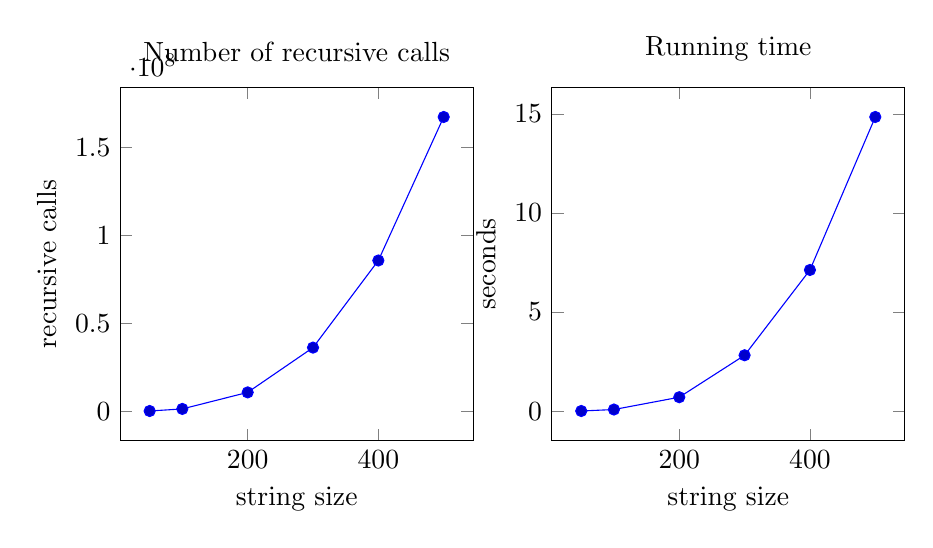
\begin{tikzpicture}
\begin{groupplot}[group style={group size=2 by 1},height=0.5\textwidth,width=0.5\textwidth]
    \nextgroupplot[title=Number of recursive calls, xlabel=string size, ylabel=recursive calls, legend pos=north west]
    \addplot coordinates {
        (50, 171256)
        (100, 1352506)
        (200, 10745006)
        (300, 36177506)
        (400, 85650006)
        (500, 167162506)};
    \nextgroupplot[title=Running time, xlabel=string size, ylabel=seconds, legend pos=north west]
    \addplot coordinates {
        (50, 0.009821)
        (100, 0.084296)
        (200, 0.705466)
        (300, 2.82136)
        (400, 7.1228)
        (500, 14.8394)};
\end{groupplot}
\end{tikzpicture}
\end{figure}
\FloatBarrier

The running time plot follows exactly the same curve as the number of recursive calls, which was expected.

Here is the verification of the complexity of the correction parser.

\begin{align*}
    &y = 1.187152 \cdot 10^{-7} \cdot x^3
\end{align*}

\FloatBarrier
\begin{figure}[h]
\centering
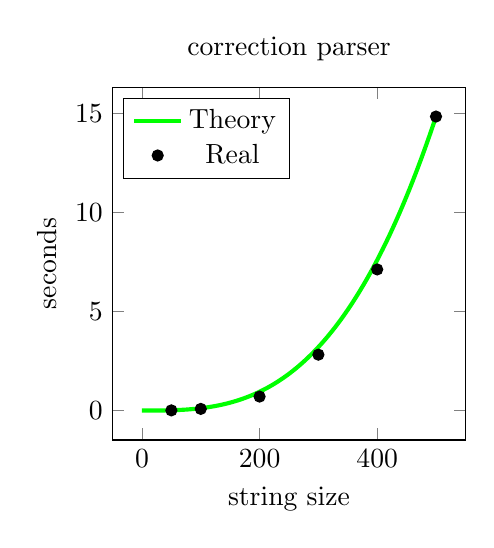
\begin{tikzpicture}
\begin{groupplot}[group style={group size=1 by 1},height=0.5\textwidth,width=0.5\textwidth]
    \nextgroupplot[title=correction parser, xlabel=string size, ylabel=seconds, legend pos=north west]
    \addplot[domain=0:500, samples=100, line width=1.5pt, green] {1.187152*(10^(-7))*(x^3)};
    \addlegendentry{Theory}
    \addplot[only marks, mark=*, mark size=2pt] coordinates {
        (50, 0.009821)
        (100, 0.084296)
        (200, 0.705466)
        (300, 2.82136)
        (400, 7.1228)
        (500, 14.8394)};
    \addlegendentry{Real}
\end{groupplot}
\end{tikzpicture}
\caption{Checking theorical fit, correction parser}
\end{figure}
\FloatBarrier

The running time behaviour of the correction parser follows exactly the theorical fit, which proves that its complexity is $O(n^3)$.

\subsection{Strings starting with an `a'}

The next expimentation is on the grammar that matches strings that start with an `a'.
With that grammar the parser follows exactly the same behaviour as before, it always need the same amount of recursive calls for a string of size $n$, no matter the pattern.

\FloatBarrier
\begin{figure}[h]
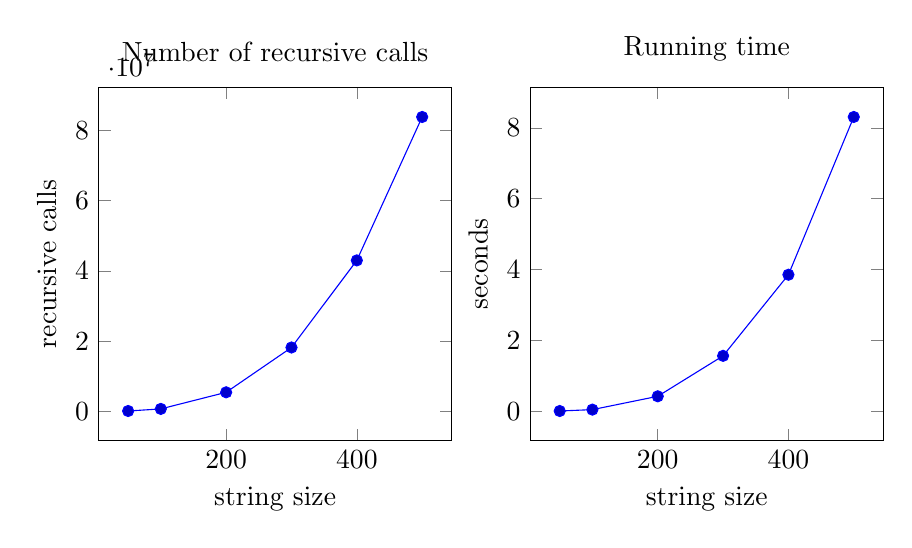
\begin{tikzpicture}
\begin{groupplot}[group style={group size=2 by 1},height=0.5\textwidth,width=0.5\textwidth]
    \nextgroupplot[title=Number of recursive calls, xlabel=string size, ylabel=recursive calls, legend pos=north west]
    \addplot coordinates {
        (50, 88005)
        (100, 686005)
        (200, 5412005)
        (300, 18178005)
        (400, 42984005)
        (500, 83830005)};
    \nextgroupplot[title=Running time, xlabel=string size, ylabel=seconds, legend pos=north west]
    \addplot coordinates {
        (50, 0.004987)
        (100, 0.04377)
        (200, 0.420274)
        (300, 1.56265)
        (400, 3.8529)
        (500, 8.30812)};
\end{groupplot}
\end{tikzpicture}
\end{figure}
\FloatBarrier

Here the parser does not need as much recursive calls as with the previous grammar but it still follows exactly the same behaviour.

The number of solved subproblems solved for this grammar follows the next sequence, with $n$ the size of the input string.

$$
1 + \dfrac{(n - 1) \cdot (3 \cdot (n - 1) + 1)}{2} + (n - 1) \cdot 2
$$

It has no use to keep going with the experimentation since no matter the grammar or the given string this parser always follows the same behaviour.


\chapter*{Conclusion}
\addcontentsline{toc}{chapter}{Conclusion}
The efficiency of the different implementations of the Cocke-Younger-Kasami algorithm depends on the used development approach for a big part but also of the given grammar.

The naive parser with its complexity of $O(3^n)$ is by far the less efficient of the implementations, there are only a few cases for which this parser can be used and compete with the others and those cases are not the cases usually met in real life.

All the other parsers are implemented using Dynamic programming and have a complexity of $O(n^3)$.
However, if with grammars in the Chomsky normal-form the two bottom-up, the top-down and the linear parsers can be more or less equivalent depending on the cases, when a linear grammar is used the linear parser is in most cases more efficient than the others.

The correction parser also has a complexity of $O(n^3)$ since it uses the top-down paradigm, but in practice it is less efficient than all the other implementations since it does more recursive calls to test different modifications.
Even if this last parser is slower than the others it can be used in way more useful ways, those kind of correction parsers are especially used in DNA and RNA analysis for example.


\listofalgorithms
\addcontentsline{toc}{chapter}{List of algorithms}

\listoffigures

\nocite{*}
\bibliographystyle{unsrt}
\bibliography{references}

\chapter*{Appendix}
\addcontentsline{toc}{chapter}{Appendix}

\section*{Grammar}

\subsection*{Grammar.h}
\lstinputlisting{code/Grammar.h}

\subsection*{Grammar.cpp}
\lstinputlisting{code/Grammar.cpp}

\section*{Abstract class parser}

\subsection*{Parser.h}
\lstinputlisting{code/Parser.h}

\subsection*{Parser.cpp}
\lstinputlisting{code/Parser.cpp}

\section*{Naive parser}

\subsection*{NaiveParser.h}
\lstinputlisting{code/NaiveParser.h}

\subsection*{NaiveParser.cpp}
\lstinputlisting{code/NaiveParser.cpp}

\section*{Top-down parser}

\subsection*{TopDownParser.h}
\lstinputlisting{code/TopDownParser.h}

\subsection*{TopDownParser.cpp}
\lstinputlisting{code/TopDownParser.cpp}

\section*{`Boolean' bottom-up parser}

\subsection*{BottomUpBoolParser.h}
\lstinputlisting{code/BottomUpBoolParser.h}

\subsection*{BottomUpBoolParser.cpp}
\lstinputlisting{code/BottomUpBoolParser.cpp}

\section*{`String' bottom-up parser}

\subsection*{BottomUpParser.h}
\lstinputlisting{code/BottomUpParser.h}

\subsection*{BottomUpParser.cpp}
\lstinputlisting{code/BottomUpParser.cpp}

\section*{Top-down correction parser}

\subsection*{TopDownParserCorrection.h}
\lstinputlisting{code/TopDownParserCorrection.h}

\subsection*{TopDownParserCorrection.cpp}
\lstinputlisting{code/TopDownParserCorrection.cpp}

\section*{Linear grammar}

\subsection*{LinearGrammar.h}
\lstinputlisting{code/LinearGrammar.h}

\subsection*{LinearGrammar.cpp}
\lstinputlisting{code/LinearGrammar.cpp}

\section*{Linear parser}

\subsection*{LinearParser.h}
\lstinputlisting{code/LinearParser.h}

\subsection*{LinearParser.cpp}
\lstinputlisting{code/LinearParser.cpp}



\end{document}
